\documentclass{book}
\usepackage[a4paper,top=2.0cm,bottom=2.0cm,left=2.0cm,right=3.0cm]{geometry}

%\documentclass[pdftex,10pt,a4paper]{book}
%\usepackage[paperwidth=19cm,
%paperheight=26cm, outer=2cm, 
%top=1.5cm, bottom=1.5cm]{ geometry}

\usepackage[english,italian]{babel} %l'ultima lingua è quella che legge per i titoli
\usepackage[utf8]{inputenc}
\usepackage[T1]{fontenc,url}
\usepackage{titlesec}
\usepackage{easylist}
\usepackage{hanging}

\usepackage[pdftex,colorlinks]{hyperref}
\hypersetup{
	colorlinks=true,
	linkcolor=black,
	filecolor=magenta,
	urlcolor=cyan,
}
\usepackage{hypcap}
\usepackage{blindtext}
\usepackage{tipa}
\usepackage{epigraph}
\usepackage{enumerate}
\usepackage{longtable}
\usepackage{setspace}
\usepackage{verbatim}
\usepackage{graphicx}
\usepackage{amsmath}
\usepackage{pbox}
\usepackage{fancyhdr}
\usepackage{cancel}
\usepackage{tabularx}
\usepackage{booktabs}
\usepackage{multirow}
\usepackage{longtable}
\usepackage{tikz}
\usepackage{tikz-qtree}
\usepackage{subfig}
\usepackage{xcolor}
\usepackage{amssymb}
\usepackage{amsmath}
\usepackage{mathrsfs}
\usepackage{textcomp}
\usepackage{circuitikz}
\usepackage{pifont}
\usepackage{imakeidx}
\usepackage{verbatim}
\usepackage{dsfont}
\usepackage{listings}
\usepackage{color}
\usepackage{upgreek}
\usepackage{tasks}
\usepackage{exsheets}
\usepackage{pgfplots}
\usepackage{amsthm}
\usepackage{wasysym}

\usepackage{tikz-cd}
\usepackage{showframe}
\renewcommand\ShowFrameLinethickness{0.15pt}
%\renewcommand*\ShowFrameColor{\color{red}}

%\usepackage{showkeys} %serve per mostrare le etichette "tag" o target, va tolta per la versione definitiva;

\SetupExSheets[question]{type=exam}

\definecolor{mygreen}{rgb}{0,0.6,0}
\definecolor{mygray}{rgb}{0.5,0.5,0.5}
\definecolor{mymauve}{rgb}{0.58,0,0.82}

\lstset{ 
  backgroundcolor=\color{white},   % choose the background color; you must add \usepackage{color} or \usepa:wckage{xcolor}; should come as last argument
  basicstyle=\footnotesize,        % the size of the fonts that are used for the code
  breakatwhitespace=false,         % sets if automatic breaks should only happen at whitespace
  breaklines=true,                 % sets automatic line breaking
  captionpos=b,                    % sets the caption-position to bottom
  commentstyle=\color{mygreen},    % comment style
  deletekeywords={...},            % if you want to delete keywords from the given language
  escapeinside={\%*}{*)},          % if you want to add LaTeX within your code
  extendedchars=true,              % lets you use non-ASCII characters; for 8-bits encodings only, does not work with UTF-8
  firstnumber=1000,                % start line enumeration with line 1000
  frame=single,	                   % adds a frame around the code
  keepspaces=true,                 % keeps spaces in text, useful for keeping indentation of code (possibly needs columns=flexible)
  keywordstyle=\color{blue},       % keyword style
  language=Octave,                 % the language of the code
  morekeywords={*,...},            % if you want to add more keywords to the set
  numbers=left,                    % where to put the line-numbers; possible values are (none, left, right)
  numbersep=5pt,                   % how far the line-numbers are from the code
  numberstyle=\tiny\color{mygray}, % the style that is used for the line-numbers
  rulecolor=\color{black},         % if not set, the frame-color may be changed on line-breaks within not-black text (e.g. comments (green here))
  showspaces=false,                % show spaces everywhere adding particular underscores; it overrides 'showstringspaces'
  showstringspaces=false,          % underline spaces within strings only
  showtabs=false,                  % show tabs within strings adding particular underscores
  stepnumber=2,                    % the step between two line-numbers. If it's 1, each line will be numbered
  stringstyle=\color{mymauve},     % string literal style
  tabsize=2,	                   % sets default tabsize to 2 spaces
  title=\lstname                   % show the filename of files included with \lstinputlisting; also try caption instead of title
}

\frenchspacing

\newcommand{\abs}[1]{\lvert#1\rvert}

\usepackage{floatflt,epsfig}

\usepackage{multicol}
\newcommand\yellowbigsqcup[1][\displaystyle]{%
  \fboxrule0pt
  \ifx#1\textstyle\fboxsep-0.6pt\else\fboxsep-1.25pt\fi
  \mathrel{\fcolorbox{white}{yellow}{$#1\bigsqcup$}}}

% definizioni
\newtheorem{teorema}{Teorema}
\newtheorem{nota}{Nota}
\newtheorem{notab}{Nota bene}
\newtheorem{attenzione}{Attenzione}
\newtheorem{definizione}{Definizione}
\newtheorem{proposizione}{Proposizione}
\newtheorem{esempio}{Esempio}
\newtheorem{esercizio}{Esercizio}
\newtheorem{osservazione}{Osservazione}
\title{Appunti geometria}
\author{Nicola Ferru}

\begin{document}
\maketitle
\tableofcontents
\listoftables
\listoffigures
\section{Premesse\dots}

In questo repository, inoltre,  sono disponibili le dimostrazioni grafiche realizzate
con \textit{Geogebra}; consiglio a tutte le persone che usufruiranno di questo lavoro, di dare un occhiata alle dimostrazioni grafiche e stare attenti,  in quanto nel tempo potranno  essere presenti delle modifiche, cosi da apportare miglioramenti al contenuto degli stessi appunti.  Solitamente il lavoro di revisione viene fatto tre/quattro volte alla settimana perché sono in piena fase di sviluppo.  Ricordo a tutti che essendo un progetto volontario ci potrebbero essere dei rallentamenti per cause di ordine superiore e quindi
potrebbero esserci meno modifiche del solito oppure essere presenti degli errori.  Chiedo pertanto  la cortesia a voi lettori di contattarmi per apportare eventuali correzioni .  Tengo a precisare che tutto il progetto è puramente open source, pertanto vengono resi disponibili i sorgenti dei file LaTex  insieme ai PDF compilati.

\begin{center}
	Cordiali saluti
\end{center}
\newpage

\section{Simboli}
\begin{multicols}{3}
	$\in$ Appartiene\\
	$\notin$ Non appartiene\\
	$\exists$ Esiste\\
	$\exists !$ Esiste unico\\
	$\subset$ Contenuto strettamente\\
	$\subseteq$ Contenuto\\
	$\supset$ Contenuto strettamente\\
	$\supseteq$ Contiene\\
	$\Rightarrow$ Implica\\
	$\Longleftrightarrow$ Se e solo se\\
	$\neq$ Diverso\\
	$\forall$ Per ogni\\
	$\ni :$ Tale che\\
	$\leq$ Minore o uguale\\
	$\geq$ Maggiore o uguale\\
	$\alpha$ alfa\\
	$\beta$ beta\\
	$\gamma$ gamma\\
	$\Gamma$ Gamma\\
	$\delta,\Delta$ delta\\
	$\epsilon$ epsilon\\
	$\sigma,\Sigma$ sigma\\
	$\rho$ rho
\end{multicols}

\chapter{Vettori}
\section{Spazio Vettoriale}
\newtheorem{SpaVet}{Spazio Vettoriale}
\begin{SpaVet}
	Uno spazio vettoriale reale (R-spazio vettoriale) è un insieme \textit{V} in
	cui sono definite un'operazione di \texttt{SOMMA} tra elementi di
	\textit{V} e un'operazione di \texttt{Prodotto tra un reale} e un elemento
	di V che soddisfano 8 proprietà:
\end{SpaVet}
\begin{enumerate}
	\item La somma è associativa quando $\forall v_1, \text{ } v_2, \text{ } v_3 
		\in V$ $\left(v_1+v_2\right)+v_3=v_1+\left(v_2+v_3\right)$;
	\item La somma è commutativa quando $\forall v_1, v_2 \in V\text{ }
		v_1+v_2=v_2+v_1$
	\item Esistenza elemento neutro 0 se e solo se $\forall v\in V \text{ }
		v+0=0+v=v$
	\item Esistenza opposto $-v$ se e solo se $\forall v \in V \text{ }
		v+(-v)=(-v)+v=0$
	\item Il prodotto per uno scalare è assoluto quando $\forall c_1,c_2 \in
		R, \forall v\in V \text{ } c_1(c_2v)=(c_1c_2)v$
	\item Il prodotto per uno scalare è distributiva quando $\forall c_1,c_2 \in
		R, \forall v\in V \text{ } (c_1+c_2)v=c_1v+c_2v$
	\item Il prodotto per uno scalare è distributiva quando $\forall c \in
		R, \forall v_1, v_2\in V \text{ }c(v_1+v_2)=cv_1+cv_2$
	\item Esistenza elemento neutro 1 quando $\forall v\in V \text{ } 1v=v$
\end{enumerate}
\begin{description}
	\item[ES:] $V_0^2\text{ } V_0^3$
	\item[ES:] $f:\mathds{R}\to \mathds{R}\text{ } x^2, \text{ } g(x)=e^x, \text{ } f(x)+g(x)=x^2+e^x\text{ } 3f(x)=3x^2$
	\item[ES:] $\mathds{R}^n$ n-uple di numeri reali
	\[
	\begin{matrix}
		\begin{bmatrix}
			x_1\\
			x_2\\
			\vdots\\
			x_n
		\end{bmatrix}+\begin{bmatrix}
			y_1\\
			y_2\\
			\vdots\\
			y_n
		\end{bmatrix}=\begin{bmatrix}
			x_1+y_1\\
			x_2+y_2\\
			\vdots\\
			x_n+y_n
		\end{bmatrix}&C\in\mathds{R} \text{ } c\begin{bmatrix}
			x_1\\
			x_2\\
			\vdots\\
			x_n
		\end{bmatrix}=\begin{bmatrix}
			cx_1\\
			cx_2\\
			\vdots\\
			cx_n
		\end{bmatrix}
	\end{matrix}
	\]
	\item[ES:] $\mathds{R}_n[x]$ polinomi di grado $\leq n$ nella variabile $x$ a coefficiente reale
		\begin{itemize}
			\item $p(x)=a_0+a_1x+a_2x^2+\dots+a_nx^n$
			\item $q(x)=b_0+b_1x+b_2x^2+\dots+b_nx^n$
		\end{itemize}
	\item[ES:] $\mathds{R}[x]$ polinomio di grado qualsiasi
		\begin{equation*}
			\begin{matrix}
				p(x)+q(x)=a_0+b_0+(a_1+b_1)x+\dots+(a_n+b_n)x^n\\
				c\in\mathds{R},\text{ } cp(x)=ca_0+ca_1x+ca_2x^2+\dots+ca_nx^n
			\end{matrix}
		\end{equation*}
\end{description}
\chapter {Numeri Complessi}
\newtheorem{NumComp}{Numeri reali}
\begin{NumComp}
	Un numero complesso è definito come un numero della forma $x+iy$, con x e y numeri reali e i una
	soluzione dell'equazione $x^2=-1$ detta unità immaginaria. i numeri reali
	sono
\end{NumComp}
\section{Operazioni con Numeri complessi}
\begin{enumerate}
\item Modulo e distanza
	\begin{equation}
		\abs{z}=\sqrt{x^2+y^2}
	\end{equation}
	Il valore assoluto (modulo) ha proprietà queste proprietà:
	\begin{equation*}
		\abs{z+w}\geq \abs{z}+\abs{w}, \text{ } \abs{zw}=\abs{z}\abs{w}, \text{ } \left|\frac{z}{w}\right|=\frac{\abs z}{\abs w}
	\end{equation*}
	Valide per tutti i numeri complessi $z$ e $w$. La prima proprietà è una versione della disuguaglianza triangolare.

\end{enumerate}
\chapter{Il determinante \label{ildet}}
In questo capitolo introdurremo uno strumento alternativo alla riduzione a gradini per determinare se le righe ({\it o le colonne}) di una matrice
siano dipendenti. Per poterne dare la definizione rigorosa, dobbiamo prima fare alcuni richiami sulle permutazioni.
\section {Richiami sulle permutazioni \label{ricsullperm}}
Dato l'insieme $\{1,2,\dots,n\}$ dei numeri naturali compresi tra 1 e $n$, per un certo $n$, una funzaione
da $\{1,2,\dots,n\}$ in se stesso associa a ogni elemento di $\{1,2,\dots,n\}$ un'immagine, scelta sempre
all'interno di $\{1,2,\dots,n\}$. Se facciamo in modo che le immagini siano tutte diverse senza
ripetizioni\footnote{\textit{Si dice la funzione è iniettiva:} una funzione iniettiva da un insieme finito in
  se stesso è automaticamente anche suriettiva, e quindi biiettiva. Richiameremo queste nozioni nel prossimo capitolo.},
queste ci daranno ancora tutti gli elementi $1,2,\dots,n$ semplicemente disposti in un altro ordine, ovvero permutati.
Si parla di {\em permutazione di n elementi.} Ad esempio, le seguenti rappresentano permutazioni di 4 elementi:
\begin{equation*}
  \begin{matrix}
    1 \to 1 & 1 \to 3\\
    2 \to 3 & 2 \to 4\\
    3 \to 2 & 3 \to 2\\
    4 \to 4 & 4 \to 1
  \end{matrix}
\end{equation*}
L'insieme delle permutazioni di $n$ elementi si denota $S_n$. Per ogni $n$, tale insieme contiene esattamente $n!:=n(n-1)(n-2)\dots 2*1$ (cioè {\it n fattoriale}) permutazioni: ad esempio, per $n = 2$ abbiamo $2!= 2 * 1 = 2$ permutazione possibili, ovvero
\begin{equation*}
  \begin{matrix}
    1 \to 1 & 1 \to 2\\
    2 \to 2 & 2 \to 1
  \end{matrix}
\end{equation*}
(tra le permutazioni vi è sempre anche anche quella che associa a ogni elemento se stesso, detta permutazione identica\footnote{Come funzione, si tratta della cosiddetta identità o funzione identica}).\\
Per $n=3$ abbiamo invece $3!=3*2*1=6$ permutazioni possibili, ovvero
\begin{equation*}
  \begin{matrix}
    1 \to 1 & 1 \to 2 & 1 \to 1 & 1 \to 3 & 1 \to 2 & 1 \to 3 \\
    2 \to 2 & 2 \to 1 & 2 \to 3 & 2 \to 2 & 2 \to 3 & 2 \to 1 \\
    3 \to 3 & 3 \to 3 & 3 \to 2 & 3 \to 1 & 3 \to 1 & 3 \to 2 \\
      p_1   &    p_2   &   p_3   &    p_4  &    p_5  &    p_6
  \end{matrix}
\end{equation*}
Si noti che $p_2, \text{ } p_3$ e $p_4$ scambiano trra loro due elementi lasciando fisso il terzo ($p_2$ scambia tra loro 1 e 2, $p_3$ scambia 2 e 3): in generale, una permutazione di questo tipo, che scambia tra loro è una trasposizione anche la prima permutazione di 4 elementi presentata all'inizio del paragrafo ({\tt scambia tra loro 2 e 3 lasciando fissi 1 e 4}), mentre la seconda non lo è.\\
Benché non tutte le permutazioni siano trasposizioni, si può dimostrare che qualunque permutazione può essere realizzata eseguendo una sequenza di trasposizioni. Ad esempio, la permutazione $p_5$ di sopra, che non è una trasposizione, può tuttavia essere ottenuta scambiando prima 1 e 2, e poi 1 e 3:
\begin{equation*}
  \begin{matrix}
    1 \to 2 \to 2\\
    2 \to 1 \to 3\\
    3 \to 3 \to 1
  \end{matrix}
\end{equation*}
ovvero può essere ottenuta componendo 2 trasposizioni.\\
In generale, se il numero di trasposizioni che servono per ottenere una permutazione data $p$ è pari, si pari, si dice che $p$ è una {\em permutazione pari}; se invece il numero di trasposizioni che servono per ottenere $p$ è dispari, si dice che $p$ è una {\em permutazione dispari}. Ad esempio, $p_5$ è una permutazione pari, in quanto l'abbiamo ottenuta componendo 2 trasposizioni; è facile vedere che anche $p_6$ è una permutazione pari, in quanto può essere ottenuta componendo due trasposizioni:
\begin{equation*}
  \begin{matrix}
    1 \to 3 \to 3\\
    2 \to 3 \to 1\\
    3 \to 1 \to 2
  \end{matrix}
\end{equation*}
Chiaramente, se una permutazione è già essa una trasposizione, allora essa è dispori ({\tt 1 è un numero dispari}).\\
Si noti che possono esserci più modi diversi di decomporre una permutazione come composizione di trasposizioni, ad esempio, la permutazione identica può essere vista o come risultato di 0 trasposizioni, oppure come risultato di 2 trasposizioni, ad esempio
\begin{equation*}
  \begin{matrix}
    1 \to 2 \to 1\\
    2 \to 1 \to 2\\
    3 \to 3 \to 3
  \end{matrix}
\end{equation*}
Tuttavia, si pu`o dimostrare che il numero di trasposizioni che servono per ottenere una permutazione data `e o sempre pari o sempre dispari ({\it nell’esempio, 0 o 2, comunque pari}).\\
Si può allora definire il \textit{segno s(p) di una permutazione p} come $s(p)=+1$ se $p$ è una permutazione dispari.\\
Siamo ora pronti a definire il determinante.
\section{La definizione di determinante}
Sia $A$ una matrice che ha $n$ righe e $n$ colonne, per qualche $n>0$: tali matrici si dicono {\it quadrate} e il numero $n$ comune a roghe e colonne si dice {\it l'ordine della matrice.} Il determinante associa a ogni matrice $A$ quadrata di ordine $n$ a entrate in un campo $\mathds{K}$ un elemento $\det(A) \in \mathds{K}$, funzione delle sue entrate, per il quale vedremo che vale l'importante proprietà che $\det(A)=0$ se e solo se la matrice ha rango minore di $n$, ovvero se e solo se le righe ({\it o le colonne}) della matrice sono dipendenti.
\begin{definizione}
  Sia A una matrice quadrata di ordine $n$ con entrate $a_{ij}$. Allora
  \begin{equation}
	\det(A)=\sum_{p\in S_n}s(p)a_{1p(1)}a_{2p(n)}
  \end{equation}
  In altrea parole, il determinante di una matrice quadrata di ordine $n$ è dato da una sommatoria che ha addendo per ogni permutazione $p\in S_n$: ognuno di questi addendi è un prodotto di entrata di $A$ del tipo $a_{1p(1)}\text{ } a_{2p(2)} \text{ \dots } a_{np(n)},$ con davanti un segno + o - a seconda che la permutazione $p$ sia pari o dispari. Si noti che l'espressione $a_{1p(1)},\text{ } a_{2p(2)}, \text{ \dots }, a_{np(n)}$ è il prodotto di $n$ entrate scelte nella matrice, una per ogni riga, con gli indici di colonna dati da $p(1),\text{ } p(2),\dots, \text{ } p(n)$: poiché una permutazione scambia gli indici $1,\text{ }2,\dots, \text{ } n$ senza ripetizioni, stiamo praticamente scegliendo un'entrata da ogni riga in modo però che le entrate scelte stiano anche su colonne diverse.
\end{definizione}
Per chiarire e illustrare la definizione precedente, consideriamo in particolare i casi $n = 2$ e $n = 3$.\\
Sia $A=\begin{pmatrix}
         a_{11} & a_{12}\\
         a_{21} & a_{22}
       \end{pmatrix}$ una matrice quadrata di ordine $n=2$. Come abbiamo visto sopra ci sono solo due permutazioni dell'insieme $\{1,2\}$ ({\tt l'identità e la trasposizione che scambia 1 con 2}) quindi nella sommatoria avremo solo due addendi, del tipo $s(p) a_{1p(1)}a_{2p(2)}$: se $p$ è l'identità, che come abbiamo osservato sopra è un permutazione pari e quindi $s(p)=+1$ e l'addendo corrispondente sarà $+a_{11}a_{22}$: se $p$ è la trasposizione che scambia 1 con 2, che è una permutazione dispari, si ha $s(p)=-1$ e l'addendo corrispondente sarà $-a_{12}a_{21}$. Il determinante di una matrice quadrata $A$ di ordine 2 risulta quindi essere
       \begin{equation}
		\det(A)=a_{11}a_{22}-a_{12}a_{21}
       \end{equation}
       Nel caso di una matrice $A= \begin{pmatrix}
                                     a_{11} & a_{12} & a_{13}\\
                                     a_{21} & a_{22} & a_{23}\\
                                     a_{31} & a_{32} & a_{33}
                                   \end{pmatrix}$ quadrata di ordine $n = 3$, la sommatoria avrà 6 addendi, tanti quante sono le permutazioni dell'insieme $\{1,2,3\}$, e per ognuna di queste permutazioni $p$ l'addendo corrispondente sarà del tipo $s(p)a_{1p(1)}a_{2p(2)}a_{3p(3)}$. Più precisamente, avremo
\begin{itemize}
\item l'addendo $+a_{11}a_{12}a_{33}$ corrispondente alla permutazione $p(1) = 1, p(2) =2, p(3) =3$ ({\tt cioè la permutazione identica, che è una permutazione pari})
\item l'addendo $-a_{11}a_{23}a_{32}$ corrispondente alla permutazione $p(1) = 1, p(2) =3, p(3) =2$ ({\tt che è una trasposizione e quindi una permutazione dispari})
\item l'addendo $+a_{12}a_{23}a_{31}$ corrispondente alla permutazione $p(1)=2,\text{ }p(2)=3,\text{ }p(3)=1$ ({\tt che è una trasposizione dispari})
\item l'addendo $-a_{12}a_{21}a_{33}$ corrispondente alla permutazione $p(1)=2,\text{ }p(2)=1,\text{ } p(3)=3$ ({\tt che è una teasposizione e quindi una permutazione dispari})
\item l'addento $+a_{13}a_{21}a_{32}$ corrispondente alla permutazione $p(1)=3,\text{ } p(2)=1,\text{ } p(3)=2$ ({\tt che si può scrivere come composizione di due trasposizioni ed è quindi una permutazione pari})
\item l'addendo $-a_{13}a_{22}a_{31}$ corrispondente alla permutazione $p(1) = 3,\text{ }p(2) = 2,\text{ }p(3)=1$ ({\tt che è una trasposizione e quindi una permutazione dispari})
\end{itemize}
e quindi si avrà, per una matrice $A$ di ordine 3: 
\begin{equation}
	\det(A)=a_{11}a_{12}a_{33}-a_{11}a_{23}a_{32}+a_{12}a_{23}a_{31}-a_{12}a_{21}a_{33}+a_{13}a_{21}a_{32}-a_{13}a_{22}a_{31}
\end{equation}
Ora, vedremo nel Paragrafo la dimostrazione del fatto che il determinante di una matrice quadratea di ordine $n$ si annulla se e solo se la matrice ha $n=2$ e $n=3$, usando le farmule esplicite ({\tt 3.2}) e ({\tt 3.3}).\\
Nel caso di una matrice $A = \begin{pmatrix} a_{11} & a_{12} \\ a_{21} & a_{22} \end{pmatrix}$ di ordine 2, essendoci solo proporzionali, ovvero diciamo che esiste un $c \in \mathds{K}$ tale che $(a_{11},a_{12})=c(a_{21}a_{22})$, cioè
\begin{equation}
	a_{11}=ca_{21},\text{ }a_{12}=ca_{22}
\end{equation}
Ma allora, moltiplicando ({\tt a entrambi i membri}) la prima uguaglianza per $a_{22}$ e la seconda per $21$ si ha $a_{11}a_{22}=ca_{21}a_{22}$ e $a_{12}a_{21}=ca_{21}a_{21}$, da cui vediamo che $a_{11}a_{22}=ca_{21}a_{22}$: quindi $a_{11}a_{22}-a_{12}a_{21}=0$, ovvero $\det(A)=0$. Quindi se una matrice di ordine 2 ha le righe proporzionali, il suo determinante è zero.\\
Viceversa, supponiamo che il determinante $a_{11}a_{22}-a_{12}a_{21}$ sia zero, ovvero
\begin{equation}
	a_{11}a_{22}=a_{12}a_{21}
\end{equation}
Supponendo per il momento che le entrate $a_{21},a_{22}$ della seconda riga non siano nulle, dividendo entrambi i membri della (3.5) per $a_{21}$ e $a_{22}$  otteniamo
\begin{equation}
	\frac{a_{11}}{a_{21}}=\frac{a_{12}}{a_{22}}
\end{equation}
cioè si ha $\frac{a_{11}}{a_{21}}=c$ e $\frac{a_{12}}{a_{22}}=c$ per qualche $c\to \mathds{K}$, da cui ritroviamo le uguaglianze ({\tt 3.4}), che $a_{21}$ e $a_{22}$ fossero entrambi diversi da zero: infatti, se ad esempio $a_{21}=0$ allora la (3.5) diventa $a_{11}a_{22}=0$, che equivale a dire che o $a_{11}=0$ oppure $a_{22}=0$: ma nel primo caso la matrice è della forma $A=\begin{pmatrix} 0 & a_{12} \\ 0 & a_{22}\end{pmatrix}$, nel secondo $A=\begin{pmatrix} a_{11} & a_{12} \\ 0 & 0\end{pmatrix}$, e in entrambi i casi otteniamo sempre che le righe sono proporzionali.\\
Nel caso di matrici di ordine 3, dimostrare che il determinante si annulla {\em se e solo se} le righe sono dipendenti, non p difficile se ci aiutiamo con un'interpretazione geometrica: {\bf infatti, prendiamo l'espressione (3.3) del determinante di una tale matrice e riscriviamola nel modo seguente:}
\begin{equation}
	a_{11}(a_{22}a_{33}-a_{23}a_{32})+ a_{12}(a_{23}a_{31}-a_{21}a_{33})+a_{13}(a_{21}a_{32}-a_{22}a_{31})
\end{equation}
Ora, le tre quantità dentro le parentesi tonde non sono altro che le componenti del prodotto vettoriale dei due vettori di $\mathds{R}^3$ dati dalla seconda e dalla terza riga della matrice:
\begin{equation*}
	R_2\wedge R_3=(a_{21},a_{22},a_{23})\wedge(a_{31},a_{32},a_{33})=(a_{22}a_{33}-a_{23}a_{32},a_{23}a_{33}-a_{21}a_{33},_{21},a_{32}-a_{22}a_{31})
\end{equation*}
Quindi la (3.7), dal momento che moltiblica le componenti di $R_1=(a_{11},a_{12},a_{13})$ con le rispettive componenti di $R_2\wedge R_3$ ({\tt la prima con la prima, la seconda con la seconda e la terza con la terza}) e somma, non è nient'altro che quello che abbiamo chiamato prodotto scalare tra $R_1$ e $R_2 \wedge R_3$. Quindi, dire che il determinante di una matrice di ordine 3 si annulla quivale a dire che le sue tre righe $R_1,R_2,R_3$ verificano l'uguaglianza.
\begin{equation}
	R_1*(R_2\wedge R_3)=0
\end{equation}
Ora, se fissiamo nello spazio $V^{3}_O$ dei vettori applicati nello spazio tridimensionali, le terne $R_1, R_2, R_3$ rappresenterano le coordinate di tre vettori applicati $\vec{OP_1}, \vec{OP_2}, \vec{OP_3}$ rispettivamente, e la (3.8) ci sta allora dicendo che il vettore $\vec{OP_1}$ è perpendicolare al vettore $\vec{OP_2}\wedge \vec{OP_3}$ ({\it infatti, abbiamo dimostrato che due vettori dello spazio sono perperndicolari solo se il prodotto scalare tra le terne dele lorfo coordinate è zero}). Ma, essendo a sua volta $\vec{OP_2}\wedge \vec{OP_3}$, per le proprietà del prodotto vettoriale, perpendicolare $\vec{OP_2}\wedge \vec{OP_3}$ significa dire che anche $\vec{OP_1}$ deve stare sul piano $p$:

\[\begin{tikzcd}
	&&& {\vec{OP_2}\wedge\vec{OP_3}} \\
	\\
	& \bullet &&&&&&&&& \bullet \\
	&&&&&& {P_3} &&&&& {\textit{p}} \\
	&&& \bullet && {} &&& {P_2} \\
	&&&&&&& {P_1} \\
	\bullet &&&&&&&&& \bullet
	\arrow[no head, from=7-1, to=3-2]
	\arrow[no head, from=7-1, to=7-10]
	\arrow[no head, from=7-10, to=3-11]
	\arrow[from=5-4, to=1-4]
	\arrow[from=5-4, to=6-8]
	\arrow[from=5-4, to=5-9]
	\arrow[from=5-4, to=4-7]
	\arrow[no head, from=3-2, to=3-11]
\end{tikzcd}\]
Quindi i tre vettori, stando sullo stesso piano, sono tra loro dipendenti, e
concludiamo che sono dipendenti anche le terne $R_1, R_2, R_3$ delle loro coordinate\footnote{Ricordiamo che dei vettori in uno spazio vettoriale sono dipendenti se e solo se lo sono, le \textit{n-uple} delle loro coordinate rispetto a una base scelta.}. Questo mostra come volevamo che il determinante di una matrice di ordine 3 si annulla se e solo se le sue riche $R_1, R_2,R_3$ sono dipendenti.\\
Nel paragrafo sulle proprietà del determinante, dimostreremo in modo puramente algebrico che questo fatto è vero per matrici di qualunque ordine. Prima di fare ciò, vediamo nel prossimo paragrafo un modo di calcolkare il determinante alternativo alla definizione, il cui utilizzo diretto richiederebbe di scrivere una sommaria che per una matrice di ordine $n$ ha $n!$ addendi, tanti quanti le permutazioni di $n$ elementi (si pensi che già per $n=4$ abbiamo $4!=24$ addendi).
\section{La formula di Laplace \label{Laplace}}
Allo scopo di calcolare il determinanete, useremo la cosiddetta \textit{formula di Laplace}, per scrivere la quale abbiamo prime bisogno di dare la seguante
\begin{definizione}
Sia $A$ una matrice quadrata di ordine $n$: per ogni entrata $a_{ij}$ di $A$, definiamo il \textit{cofattore di $a_{ij}$}, denotato $C_{ij}$, come il determinante della matrice di ordine $n-1$ che si ottiene da $A$ cancellando la riga $i$ e la colonna $j$, moltiplicato per $(-1)^{i+j}$
\end{definizione}
Vediamo subito un esempio: consideriamo la matrice di ordine 3 seguente
\begin{equation*}
  \begin{pmatrix}
    1 & 2 & 4 \\
    4 & 5 & 6 \\
    7 & 8 & 9
  \end{pmatrix}
\end{equation*}
L'entrata $a_{11}$ è uguale a 1: il suo cofattore $C_{11}$ è, in base alla definizione <++>, il determinante della matrice di ordine 2 che si ottiene cancellando la prima riga e la prima colonna (ovviamente la riga e la colonna dell-entrata $a_{11}$ presa in considerazione) moltiplicato per $(-1)^{1+1}$:
\begin{equation*}
	C_{11}=(-1)^{1+1}\det\begin{pmatrix} 5 & 6\\ 8 & 9 \end{pmatrix} = (-1)^2(5*9-6*8)=+(45-48)=-3
\end{equation*}
Invece, se per esempio prendiamo l'entrata $a_{23}=6$, il suo cofattore $C_{23}$ è il determinante della matrice di ordine 2 che si ottiene cancellando la seconda riga e la terza colonna (ovvero la riga e la colonna dell'entrata $(-1)^{2+3}$):
\begin{equation*}
	C_{11}=(-1)^{1+1}\det\begin{pmatrix} 1 & 2 \\ 7 & 8 \end{pmatrix} = (-1)^5(1*8-2*7)=-(8-14)=+6
\end{equation*}
Siamo ora pronti a enunciare il seguante risultato, sche ci dà una formula per il calcolo del determinante di una matrice:
\begin{proposizione}
  Sia $A$ una matrice di ordine $n$. Data una sua qualunque riga $\begin{pmatrix} a_{i1} & a_{i2} & \dots & a_{in} \end{pmatrix}$ o una qualungue colonna $\begin{pmatrix} a_{1j} \\ a_{2j} \\ \vdots \\ a_{nj} \end{pmatrix}$, si ha
  \begin{eqnarray}
    \det(A)=a_{i1}C_{i1}+a_{i2}C_{i2}+\dots+a_{in}C_{in}\\
    \det(A)=a_{1j}C_{1j}+a_{2j}C_{2j}+\dots+a_{nj}C_{nj}
  \end{eqnarray}
  La proposizione, che non dimostriamo, afferma quindi che il determinante di una matrice si può calcolare scegliendo una riga o una colonna, moltiplicando ogni elemento della riga o della colonna per il suo cofattore e sommando il tutto. La (3.9) e la (3.10) si dicono rispettivamente \textit{formula (o sviluppo) di Laplace secondo la i-esima riga e la la formula (o sviluppo) di Laplace secondo la j-esima colonna.}\\
  L'osservazione importante da fare sulla formula di Laplace è che essa esprime il determinante di una matrice di ordine $n$ in funzione dei suoi cofattori, che sono, a parte il fattore $(-1)^{i+j}$, determinanti di matrici di ordine $n-1$: a loro volta, potremo poi calcolare ciascuno di questi cofattori riutilizzando la formula di Laplace, con la quale ci ridurremo a calcolare determinanti di matrici di oridne $n - 2$, e così viam fino a che non arriveremo a matrici di ordine 2 per le quali la formula del determinante è particolarmente semplice da ricordare. Vediamo un esempio.
\end{proposizione}
\begin{esempio}
  Sia $A=\begin{pmatrix} 1 & 1 & 0 & 0 \\ 0 & 1 & -1 & 1 \\ 1 & 0 & 0 & 1 \\ 1 & 2 & 1 & 0\end{pmatrix}$. Scegliamo di sviluppare il determinante secondo Laplace rispetto alla terza riga, usando cioè la formula (3.9) nel caso $i = 3$:
  \begin{equation*}
    \det (A)=a_{31}C_{31}+a_{32}C_{32}+a_{33}C_{33}+a_{34}C_{34}.
  \end{equation*}
  Per definizione di cofattori e tenendo conto che $a_{32}=a_{33}=0$ (e quindi non abbiamo bisogno di calcolare i corrispondenti cofattori) si ha
  \begin{equation}
	\det(A)=1*(-1)^{3+1}\det\begin{pmatrix} 1 & 0 & 0 \\ 1 & -1 & 1 \\ 2 & 1 & 0\end{pmatrix} + 1*(-1)^{3+4}\det\begin{pmatrix} 1 & 1 & 0 \\ 0 & 1 & -1 \\ 1 & 2 & 1\end{pmatrix}
  \end{equation}
  Ora, cisascuno dei due determinanti di ordine 3 che compaiono in questa uguaglianza può essere calcolato usando di nuovo la formula data. Ad esempio, se per il primo determinante scegliamo la terza colonna (quindi dobbiamo usare $\det (A)=a_{11}C_{11}+a_{12}C_{12}+a_{13}C_{13}$) tenendo conto che $a_{13}=0$, si ha
  \begin{equation*}
	\det\begin{pmatrix} 1 & 0 & 0 \\ 1 & -1 & 1 \\ 2 & 1 & 0\end{pmatrix}=1*(-1)^{2+3}\det\begin{pmatrix} 1 & 0 \\ 2 & 1 \end{pmatrix}=-1.
  \end{equation*}
  dove il determinante di ordine 2 è stato calcolato usando la formula $\det(A)=a_{11}a_{22}-a_{12}a_{21}$.
  Analohgalmente, se per l'altro determinante scegliamo la prima riga (quindi dobbiamo usare
  $\det (A)=a_{11}C_{11}+a_{12}C_{12}+a_{13}C_{13}$) tenendo conto che $a_{13}=0$, si ha
  \begin{equation*}
    \det\begin{pmatrix} 1 & 1 & 0 \\ 0 & 1 & -1 \\ 1 & 2 & 1\end{pmatrix}=1*(-1)^{1+1}\det\begin{pmatrix} 1 & -1 \\ 2 & 1 \end{pmatrix} + 1 * (-1)^{3+1}\det\begin{pmatrix} 0 & -1 \\ 1 & 1\end{pmatrix} =3-1=2.
  \end{equation*}
  Sostituendo questi risultati nella (3.11), si trova allora
  \begin{equation*}
    \det(A)=1*(-1)^{3+1}(-1)+1*(-1)^{3+4}2=-3.
  \end{equation*}
  Nell'enunciato del Proposizione \ref{Laplace}, è sottointeso il fatto che il risultato dello sviluppo ci darà sempre il determinante di $A$ indipendentemente dalla riga o colonna scelta: questo è molto importante nella pratica in quanto ci consente, come visto anche nell-esempio, di scegliere se possibile righe o colonne in cui alcune in cui alcune entrate siano nulle, così da non dover calcolare i corrispondente cofattori. 
\end{esempio}
\begin{osservazione}
  Notiamo che l'espressione (3.7), che abbiamo usato per mostrare geometricamente che il determinante di una matrice di ordine 3 si annulla se e solo se le sue righe sono dipendenti, non era altro che lo sviluppo di Laplace di tale determinante rispetto alla prima riga: infatti, ricordando la derinizione di determinante di una matrice di ordine 2, si trava
  \begin{equation*}
	\begin{matrix}
          a_{11}(a_{22}a_{33}-a_{23}a_{32})-a_{12}(a_{21}a_{33}-a_{23}a_{31})+a_{12}(a_{21}a_{32}-a_{22}a_{31})=\\
          a_{11}(-1)^{1+1}\det\begin{pmatrix} a_{22} & a_{23} \\ a_{32} & a_{33}\end{pmatrix}+a_{12}(-1)^{1+2}\det\begin{pmatrix} a_{21} & a_{23} \\ a_{31} & a_{33}\end{pmatrix}+a_{13}(-1)^{1+3}\det\begin{pmatrix} a_{21} & a_{22} \\ a_{32} & a_{32}\end{pmatrix}=\\a_{11}C_{11}+a_{12}C_{12}+a_{13}C_{13}
        \end{matrix}
  \end{equation*} 
\end{osservazione}
\section{Proprietà del determionante}
In questo paragrafo dimostreremo finalmente che il determinante di una matrice $A$ si annulla \underline{se e solo se} le sue righe sono dipendenti. A questo scopo, iniziamo con l'enunciazione e dimostrazione tre importanti proprietà del determinante:
\begin{enumerate}
\item se $A^\prime$ si ottiene da $A$ moltipricando una riga di $A$ per $c\in \mathds{K}$, allora $\det(A^\prime)=c\det(A)$\\
  Ad esempio, se $A=\begin{pmatrix} 1 & 2 \\ 3 & 4 \end{pmatrix}$ e $A^\prime =\begin{pmatrix} 5 & 10 \\ 3 &4 \end{pmatrix}$ è la matrice ottenuta da $A$ moltiplicando la prima riga per $c=5$, ho $\det(A^\prime)=5*4-10*3=5\det (A)$.\\
  In altre parole, se una riga di una matrice viene moltiplicata per una scala $c$, quando calcoliamo il determinante possiamo ``portare fuori'' questo scalare.\\
  In base alle definizione ({\it <++>}) di determinantem, il determinante della matrice $A^\prime$ in cui abbiamo moltiplicato tutti gli elementi della riga \textit{i-esima} per $c$ è $\det (A^\prime)=\sigma s(p)a_{1p(1)}\dots(ca_{ip(1)})\dots a_{np(n)}$: essendo il fattore $c$ comune a tutti gli addendi della sommatoria, possiamo metterlo in evidenze in eveidenza alla somma e scivere $\det(A^\prime) = c \sigma s(p)a_{ip(n)}a_{1np(n)}$, ovvero $\det(A^\prime)=c\det(A)$, come volevamo.
\item supponiamo di sommare a una riga $R_i$ di una matrice $A$ una \textit{n-upla} $v=(v_{i1},v_{i2},\dots,v_{in})$. Allora, il determinante della nuova matrice $A^\prime$ così ottenuta vale
  \begin{equation}
    \det(A^{\prime})=\det(A)+\det\begin{pmatrix} R_1 \\ \dots \\ v\\ \dots \\ R_n \end{pmatrix}
  \end{equation}
  dove stiamo denotando con $\begin{pmatrix} R_1 \\ \dots \\ v\\ \dots \\ R_n \end{pmatrix}$ la matrice ottenuta da $A$ sostituendo $v$ al posto della riga $R_i$. Possiamo anche scrivere
  \begin{equation}
	\det\begin{pmatrix} R_1 \\ \dots \\ R_i+v\\ \dots \\ R_n \end{pmatrix}=\det\begin{pmatrix} R_1 \\ \dots \\ R_i\\ \dots \\ R_n \end{pmatrix}+\det \begin{pmatrix} R_1 \\ \dots \\ v\\ \dots \\ R_n \end{pmatrix}
  \end{equation}
  Ad esempio, consideriamo la matrice $A=\begin{pmatrix} 1 & 2 \\ 2 & 1 \end{pmatrix}$ e sommiamo
  alla sua seconda riga (2, 1) la coppia (1, 3), ottenendo  $A=\begin{pmatrix} 1 & 2 \\ 3 & 4 \end{pmatrix}$. Allora si ha proprio
  \begin{equation*}
	\det(A^\prime)=\det\begin{pmatrix} 1 & 2 \\ 3 & 4 \end{pmatrix}=\det(A)+\begin{pmatrix} 1 & 2 \\ 1 & 3 \end{pmatrix}
  \end{equation*}
  ovvero $-2=-3+1$.
		\begin{proof}
			Se $R_i=\begin{pmatrix}a_{i1} & a_{i2} & \dots & a_{in}\end{pmatrix}$
			allora la riga i-esima della matrice\\
			$A^\prime$ è $R_i+v+\begin{pmatrix}a_{i1}+v_{i1} & a_{i2}+v_{i2} & 
			\dots & a_{in}+v_{in}\end{pmatrix}$
			In base alla definizione (<++>) di determinante, si ha
			$\det(A^\prime)=\sum s(p)a_{ip(1)}\dots (a_{ip(i)}+v_{ip(i)})\dots a
			_{np(n)}=\sum s(p)a_{ip(1)}\dots a_{ip(i)}\dots a_{np(n)}+\sum s(p)a
			_{ip(1)}\dots v_{ip(i)}\dots a_{np(n)}$ ovvero 
			$\det(A)+\det\begin{pmatrix}R_1\\ \dots\\ v\\ \dots\\ 
			R_n\end{pmatrix}$, come volevamo.
		\end{proof}
    \item se $A^\prime$ si ottiene da $A$ scambiando tra loro due righe allora $\det(A^\prime)=-\det(A)$\\
		Ad esempio, se $A=\begin{pmatrix} 1 & 2 \\ 3 & 4 \end{pmatrix}$ e
			  $A^{\prime}=\begin{pmatrix} 4 & 3 \\ 1 & 2 \end{pmatrix}$ è la
			  matrice ottenuta da $A$ scambiando tra loro la prima e la seconda
			  riga, ho $\det(A)=1*4-2*3=-2$ e $\det(A^\prime)=3*2-4*1=+2$.
		\begin{proof}
			Sia $A^\prime$ la matrice ottenuta da $A$ scambiando la riga $R_i$
			con la $R_j$: quindi per ogni $k$ si ha $a^\prime_{ik}=a_{jk}$ e
			$a^\prime_{jk}=a_{ik}$, mentre tutte le altre sono uguali a quelle
			di $A$.\\
			Quindi, in base alla (3.1), si ha
			\begin{equation}
				\det(A^\prime) = \sum_{p\in Sn} s(p) a^\prime_{1p(1)}\dots
				a^\prime_{ip(i)}\dots a^\prime_{jp(j)}\dots a^\prime_{np(n)} =
				\sum_{p\in Sn} s(p) a^\prime_{1p(1)}\dots
				a^\prime_{jp(j)}\dots a^\prime_{ip(i)}\dots a^\prime_{np(n)}.
			\end{equation}
			(in pratica, l'unica differenza tra la (3.14) e l'espressione del
			determinante di $A$ è che in ogni addendo le entrate ``centrali''
			habbi gli indici di riga $i$ e $j$ scambiati tra logo).\\
			Ora, allo scopo di dimostrare il risultato, riscriviamo la (3.14)
			come segue: consideriamo la trasposizione $\mathcal{T}\in S_n$ che
			scambia $i$ con $j$ e lascia invariati tutti gli altri elementi:
			quindi $j=\mathcal{T}(i), \text{ } i=\mathcal{T}(j)$, e per tutti
			gli altri indici $k =\mathcal{T}(k)$.\\
			Allora possiamo scrivere
			\begin{equation}
				\det(A^\prime) = \sum_{p\in Sn} s(p) a_{1\mathcal{T}(1)}\dots
				a^\prime_{jp\mathcal{T}(j)}\dots a^\prime_{ip\mathcal{T}(i)}
				\dots a^\prime_{np\mathcal{T}(n)} 
			\end{equation}
			Ora, per un qualunque indice $k$, si ha che $p(\mathcal{T}(k))$ è
			il valore associato a $k$ dalla permutazione $p \mathcal{T}$ che si
			ottiene componendo $p$ con $\mathcal{T}$ (ovvero applicando, da
			destra, prima $\mathcal{T}$ e poi $p$). Tale permutazione è tale
			dispari, e di un numero pari di trasposizione (una in più di $p$),
			e analogamente se dispari di trasposizione, e allora
			$p\mathcal{T}$, sarà composta da un numero dispari di trasposizione
			(una in più di $p$), e analogamente se $p$ è dispari vuol dire che
			si scrive come composizione di un numero di strasposizioni.
			Riassumendo, la (3.15), scambiando anche di ordine i due fattori
			centrali $a_{j p\mathcal{T}(j)}$ e $a_{ip\mathcal{T}(i)}$ in ogni
			addendo (il prodotto gode della proprietà commutativa) può essere
			scritta nel modo seguente
			\begin{equation}
				\det(A^\prime) = -\sum_{p\in S_n} s(p\mathcal{T})
				a_{1p\mathcal{T}(1)} \dots a_{i p\mathcal{T}(i)} \dots a_{j
				p\mathcal{T}(j)} \dots a_{n p\mathcal{T}(n)}
			\end{equation}
			Ora, quest'ultima espressione, con il segno meno davanti, è uguale
			a quella del determinante di $A$ a parte che in essa compare
			$p\mathcal{T}$ invece che $p$. Ma in realtà questo non cambia
			nulla, in quanto facciamo variare $p$ tra tutti le permutazioni
			$p_1,p_2,\dots,p_{n!}$ di $n$ elementi, $p_1\mathcal{T},
			p_2\mathcal{T},\dots,p_{n!}\mathcal{T}$ sono ancora {\em tutte} le
			permutazioni: per non esserlo, dovrebbe infatti succedere che
                        $p_i\mathcal{T}=p_j\mathcal{T}$ allora
                        $p_i\mathcal{T}\mathcal{T}=p_j\mathcal{T}\mathcal{T}$, ovvero, essendo
                        $\mathcal{T}\mathcal{T}=id,p_i=p_j$.\\
                        Quindi, a parte il segno, la ({\bf 3.16}) contiene esattamente un
                        addendo per ogni permutazione, e otteniamo il risultato voluto.
		\end{proof}
\end{enumerate}
\clearpage              
La proprietà (3) ha l'importante conseguenza che se una matrice ha due {\it righe uguali allora
  il suo determinante è nullo.}\\
Infatti, in base alla (3) se $A^\prime$ è ottenuta da $A$ scambiando tra loro due righe allora
$det(A^\prime)=-det(A)$, ma se le righe scambiate sono proprio le due righe uguali allora
$A^\prime=A$, da cui concludiamo $det(A)=-det(A)$, ovvero $det(A)=0$. Combinando questo fatto
con le proprietà (2) e (1) possiamo capire come si comporta il determinante quando eseguiamo
operazioni elementari del terzo tipo: infatti, supponiamo che $A^\prime$ sia ottenuta da $A$
sommanda alla sua {\it i-esima} riga $R$, la {\it j-esima} riga $R_j$ moltiplicata per $c$,
ovvero $A^\prime =\begin{pmatrix}
R_1\\
\dots\\
R_i +cR_j\\
\dots\\
R_j\\
\dots\\
R_n
\end{pmatrix}
$.\\
Ma allora, per la proprietà (2) e la proprietà (1) ho
\begin{equation}
  \det(A^\prime)=\det\begin{pmatrix}
                     R_1\\
                     \dots\\
                     R_i +cR_j\\
                     \dots\\
                     R_j\\
                     \dots\\
                     R_n
                   \end{pmatrix}=\det
                   \begin{pmatrix}
                     R_1\\
                     \dots\\
                     R_i\\
                     \dots\\
                     R_j\\
                     \dots\\
                     R_n
                   \end{pmatrix}+\det
                   \begin{pmatrix}
                     R_1\\
                     \dots\\
                     cR_j\\
                     \dots\\
                     R_j\\
                     \dots\\
                     R_n
                   \end{pmatrix}=\det
                   \begin{pmatrix}
                     R_1\\
                     \dots\\
                     R_i\\
                     \dots\\
                     R_j\\
                     \dots\\
                     R_n
                   \end{pmatrix}+c\det
                   \begin{pmatrix}
                     R_1\\
                     \dots\\
                     R_j\\
                     \dots\\
                     R_j\\
                     \dots\\
                     R_n
                   \end{pmatrix}
\end{equation}
Ma mentre i primo addendo dopo l'ultima uguaglianza è il determinante della matrice $A$, il
secondo addendo è nullo, in quanto determinante di una matrice con le righe uguali (compare
due volte $R_j$). Quindi la (3.17) si legge come
\begin{equation*}
  \det(A^\prime)=\det(A)+0=\det(A).
\end{equation*}
Ora siamo finalmente pronti a dimostrare il
\begin{teorema}
  Una matrice $A$ quadrata di ordine $n$ ha rango $n$ (ovvero ha le righe indipendenti) se e
  solo se $det (A)\neq 0$.
  \begin{osservazione}
    per sapere se $n$ vettori di $\mathds{R}^\prime$ sono linearmente indipendenti oppure
    dipendenti, si dispongono le loro coordinate in una matrice e si calcola il determinante.
    \begin{itemize}
    \item Se $\det \neq 0$, allora i vettori sono lineari indipendenti.
    \item Se $\det = 0$, allora i vettori sono lineari dipendenti.
    \end{itemize}
  \end{osservazione}
  \begin{proof}
    Supponiamo che $A$ abbia rango massimo $n$. Allora, come sappiamo, nella matrice $A^\prime$ si
    ottiene da A mediante operazioni elementari, e come abbiamo visto sopra le operazioni
    elementari o non modificano il determinante ({\it terzo tipo}) o lo cambiano di segno (prima
    tipo) o lo moltiplicano per un coefficiente non nullo (secondo tipo), si avrà
    $\det(A^\prime)=\pm c_1\dots c_m\det (A)$, con $c_1,\dots,c_m\neq 0$, e per dimostrare che
    $\det(A^\prime)\neq 0$.\\
    Poiché stiamo dicendo che matrice quadrata a gradini senza righe nulle, $A^\prime$ è della
    forma
    \begin{eqnarray*}
      A^\prime=\begin{pmatrix}
                 a^\prime_{11} & a^\prime_{12} & \dots &a^\prime_{1n-1}& a^\prime_{1n}\\
                 0           & a^\prime_{22} & \dots &a^\prime_{2n-1}& a^\prime_{2n}\\
                               && \vdots\\
                 0 & 0 & \dots &a^\prime_{n-1n-1}& a^\prime_{n-1n}\\
                 0 & 0 & \dots & 0 & a^\prime_{nn}
               \end{pmatrix} & \begin{matrix}
                                 \text{Triangolare superiore con}\\
                                 \text{elementi sulla diagonale tutti}\\
                                 \text{diversi da zero}
                                 \end{matrix}
    \end{eqnarray*}
    con $a^\prime_{11},a^\prime_{12},\dots,a^\prime_{n-1n-1}, a^\prime_{nn}$ tutti divensi da zero.
    Calcoliamo il determinante di $A^\prime$ sviluppando secondo Laplace rispetto alla prima
    colonna: essendo $a^\prime_{11}$ l'unico elemento non nullo, si avrà
    \begin{equation*}
      \det(A^\prime)=a^\prime_{11}(-1)^{1+1}\det\begin{pmatrix}
                                                  a^\prime_{22} & \dots &a^\prime_{2n-1}
                                                  & a^\prime_{2n}\\
                               		          && \vdots\\
                  0 & \dots &a^\prime_{n-1n-1}& a^\prime_{n-1n}\\
                                                  0 & \dots & 0 & a^\prime_{nn}
                                                \end{pmatrix}
    \end{equation*}
    \clearpage
    Se sviluppiamo ora il cofattore di nuovo secondo Laplace rispetto alla sua prima colonna,
    che ha come unico elemento non nullo $a_{22}^\prime$, otteniamo
    \begin{equation*}
      \det(A^\prime)=a^\prime_{11}(-1)^{1+1}\det\begin{pmatrix}
                                                  a^\prime_{33} & \dots &a^\prime_{3n-1}
                                                  & a^\prime_{2n}\\
                               		          && \vdots\\
                  0 & \dots &a^\prime_{n-1n-1}& a^\prime_{n-1n}\\
                                                  0 & \dots & 0 & a^\prime_{nn}
                                                \end{pmatrix}
    \end{equation*}
    e continuando a sviluppare sempre rispetto alla prima colonna otteniamo $\det (A^\prime)=
    a^\prime_{11}a_{12}^\prime\dots a_{nn}^\prime$. Essendo come abbiamo detto qgli elementi
    $a^\prime_{11},a_{12}^\prime,\dots, a_{nn}^\prime$ tutti non nulli, si ha, come volevamo,
    $\det(A^\prime)\neq 0$: la prima implicazione è dimostrata.
    \begin{osservazione}
      il $\det$ diuna matrice triangolare è il prodotto degli elementi sulla diagonale
    \end{osservazione}
    Per quello che riguarda l'implicazione inversa se $\det (A)\neq 0$ allora $A$ ha rango $n$,
    essa si dimostra facilmente per assurdo osservando che se $A$ non avesse rango $n$, allora
    la matrice ridotta $A^\prime$ avrebbe una riga nulla, e sviluppando il suo determinante
    secondo Laplace proprio rispetto a quella riga otterremmo $\det(A^\prime) = 0$ (in quanto ogni
    sviluppo andrebbe moltiplicato per zero). ma poiché come abbiamo osservato nel dimostrare la
    prima implicazione il determinante della matrice ridotta è nullo se e solo se lo è quello
    della matrice di partenza, allora avremmo anche $\det(A)=0$, contro l'ipotesi.
  \end{proof}
  \begin{osservazione}
    Nell'osservazione <++> abbiamo visto un modo per passare da equazioni parametriche di un
    piano alla sua equazione cartesiana mediante eliminazione dei parametri $t$ e $s$ per
    sostituzione. Vediamo ora che grazie al determinante esiste un procedimento più elegante:
    le equazioni parametriche (\ref{eqpar}) possono essere riscritte nel seguente modo:
    \begin{equation*}
      \begin{pmatrix}
        x\\
        y\\
        z
      \end{pmatrix}
      =\begin{pmatrix}
         x_0\\
         y_0\\
         z_0
       \end{pmatrix}
       +t\begin{pmatrix}
           l\\
           m\\
           n
         \end{pmatrix}
         +s\begin{pmatrix}
            l^\prime\\
            m^\prime\\
            n^\prime
          \end{pmatrix}
    \end{equation*}
    ovvero
    \begin{equation*}
      \begin{pmatrix}
        x-x_0\\
        y-y_0\\
        z-z_0
      \end{pmatrix}=t\begin{pmatrix}
                       l\\
                       m\\
                       n
                     \end{pmatrix} +s
                     \begin{pmatrix}
                       l^\prime\\
                       m^\prime\\
                       n^\prime
                     \end{pmatrix}.
    \end{equation*}
    Quest'ultima ugualianza ci dice che il vettore $(x-x_0,y-y_0,z-z_0)$ si scrive come
    combinazione lineare di $(l,m,n)$ e $(l^\prime,m^\prime,n^\prime)$, e quindi che la matrice
    \begin{equation*}
      \begin{pmatrix}
        x-x_0 & l &l^\prime\\
        y-y_0 & m &m^\prime\\
        z-z_0 & n & n^\prime
      \end{pmatrix}
    \end{equation*}
    che ha tale vettore come colonne ha rango 2. Questo, per la proprietà appena dimostrata che
    afferma che una matrice quadrata di ordine n ha rango minore di n se e solo se il suo
    determinate è zero, equivale a dire che
    \begin{equation*}
      \det\begin{pmatrix}
        x-x_0 & l &l^\prime\\
        y-y_0 & m &m^\prime\\
        z-z_0 & n & n^\prime
      \end{pmatrix}=0
    \end{equation*}
    Sviluppando questo determinante, si ottiene quindi un'equazione in $x,y,z$ che è appunto
    l'equazione cartesiana del piano.
    \begin{esempio}
      supponiamo che il piano abbia equazioni parametriche $
      \begin{cases}
        x=1+t+s\\
        y=2-t+2s\\
        z=3+t-s
      \end{cases}
      $.
    \end{esempio}
    Allora, la sua equazione cartesiana è data da
    \begin{equation*}
      \det
      \begin{pmatrix}
        x-1 & 1 &1\\
        y-2 &-1 & 2\\
        z-3 &1 & -1
      \end{pmatrix}
    \end{equation*}
    ovvero, sviuppando per sempio secondo Laplace rispetto alla prima colonna,
    \begin{equation*}
      (x-1)\det
      \begin{pmatrix}
        -1 & 2\\
        1 & -1
      \end{pmatrix} -(y-2) \det
      \begin{pmatrix}
        1 & 1 \\
        1 & -1
      \end{pmatrix}+(z-3)\det
      \begin{pmatrix}
        1 &1 \\
        1 &-1
      \end{pmatrix}=0
    \end{equation*}
    \clearpage
    cioè, svolgendo i calcoli,
    \begin{equation*}
      -(x-1)+2(y-2)+3(z-3)=-x+2y+3z-12=0
    \end{equation*}
    Nel caso in cui il piano sia quello passante per tre punti non allineati di coordinate
    $(x_0,y_0,z_0),(x_1,y_1,z_1),$\\$(x_2,y_2,z_2)$, abbiamo visto nella (<++>) che in tal caso basta
    prendere $(l,m,n)=(x_1-x_0,y_1-y_0,z_1-z_0)$ e $(l^\prime,m^\prime,n^\prime)=
    (x_2-x_0,y_2-y_0,z_2-z_0)$, e quindi la (<++>) diventa
    \begin{equation}
      \det
      \begin{pmatrix}
        x-x_0 &x_1-x_0 & x_2-x_0\\
        y-y_0 & y_1-y_0 & y_2-y_0\\
        z-z_0 & z_1-z_0 & z_2-z_0
      \end{pmatrix}=0
    \end{equation}
    che ci da un modo per scrivere subito l'equazione cartesiana del piano che passa per i tre
    punti.
  \end{osservazione}
  \begin{osservazione}
    Tutti le proprietà del determinante che abbiamo visto valide per operazioni sulle righe sono
    vere anche se effettuiamo le stesse operazione sulle colonne, ovvero:
    \begin{enumerate}
    \item se $A^\prime$ si ottiene da $A$ moltiplicando una colonna di $A$ per $c\in \mathds{K}$,
      allora $\det(A^\prime)=c\det(A)$
      \begin{esempio}
        se $A=
        \begin{pmatrix}
          1 & 2\\
          3 & 4
        \end{pmatrix}
        $ e $A^\prime=
        \begin{pmatrix}
          5 & 2\\
          15 & 4
        \end{pmatrix}
        $ è la matrice ottenuta da $A$ moltiplicando la prima colonna per $c = 5$, ho $\det(A)=-2$
        e $\det(A^\prime)=5\times4-10\times3=-10=5\det(A)$.
      \end{esempio}
    \item se a una colonna $C_i$ di una matrice $A$ sommiamo una $n$-upla data $v$ (scritta in
      colonna) si ha
      \begin{equation*}
        \det(A^\prime)=\det(A)+\det
        \begin{pmatrix}
          C_i & \dots & v & \dots & C_n
        \end{pmatrix}
      \end{equation*}
      \begin{esempio}
        se alla seconda colonna $C_2$ della matrice $
        A=\begin{pmatrix}
            1 & 2 \\
            3 & 1 
        \end{pmatrix}
        $ sommiamo la coppia $v=
        \begin{pmatrix}
          0 \\
          3
        \end{pmatrix}
        $, ottenendo così $C^\prime_2=C_2+v=
        \begin{pmatrix}
          2 \\
          1
        \end{pmatrix} +
        \begin{pmatrix}
          0 \\
          3
        \end{pmatrix} =
        \begin{pmatrix}
          2\\
          4
        \end{pmatrix}
        $, si ha
        \begin{equation*}
          \det
          \begin{pmatrix}
            1 & 2\\
            3 & 4
          \end{pmatrix} =
          \det\begin{pmatrix}
                1 & 2 \\
                3 & 4
          \end{pmatrix} + \det
          \begin{pmatrix}
            1 &0\\
            3 &3
          \end{pmatrix}
        \end{equation*}
        come può verificato calcolando i determinanti (si ottiene $-2=-5+3$).
      \end{esempio}
    \item se $A^\prime$ si ottiene da $A$ scambiando tra loro due colonne, allora $\det(A^\prime)
      =-\det(A)$
      \begin{esempio}
        se
        $
          A=\begin{pmatrix}
            1 & 2\\
            3 & 4
          \end{pmatrix}
        $ e
        $
          A^\prime=
          \begin{pmatrix}
            2 & 1\\
            4 & 3
          \end{pmatrix}$
        è la matrice ottenuta da $A$ scambiando tra loro la prima e la seconda colonna,
        ho $\det(A)=1*4-2*3=-2$ e $\det(A^\prime)=2*3 -1* 4=+2$.       
      \end{esempio}
      Omettiamo la dimostrazione di queste tre proprietà.
    \end{enumerate}
    Concludiamo questo capitolo mostrando come, benché non si possa calcolare il determinante di
    una matrice non quadrata, il determinante posso comunque essere usato per calcolare il rango
    di qualunque matrice.\\
    Più precisamente, data una matrice $A$, chiamiamo {\it sottomatrice di} $A$ una matrice che si ottiene da $A$
    scegliendo alcune righe e alcune colonne e cancellando le rimanenti. 
  \end{osservazione}
  \begin{esempio}
    se $A=
    \begin{pmatrix}
      0 & 1 & 1 &1 \\
      1 & 2 & 2 & 3 \\
      -1 & 0 &0 & -1
    \end{pmatrix}
    $, allora scegliendo la prima e la terza riga, e tra la quarta colonna\footnote{ovvero cancellando la seconda
    riga e le prime due colonne} si ottiene la sotto matrice $
  \begin{pmatrix}
    1 &1 \\
    0 & -1 
  \end{pmatrix}
  $
  \end{esempio}
\end{teorema}
    
\chapter{Applicazione lineari e prodotto di matrici}
\section{Applicazioni lineari: definizione e esempi\label{applin}}
Inizieremo ora a parlare di funzioni tra spazi vettoriali. Ricordiamo che una funzione $f:X\to Y$ tra due insiemi
$X$ (detto \textit{dominio}) e $Y$ (detto \textit{codominio}) è una legge che associa a ogni $x\in X$ un ben
preciso elemento di $Y$, detto \textit{immagine di $x$} e denotato $f(x)$.\\
Noi studiaeremo le funzioni $f:V\to W$ in cui dominio e codominio $V$ e $W$ sono spazi vettoriali su un certo
campo $\mathds{K}$, e in particolare studieremo quelle che soddisfano la seguente
\begin{definizione}
  Una funzione $f:V\to W$ tra spazi vettoriali si dice \texttt{funzione lineare} (o \textit{applicazione
    lineare}) se verifica le due seguenti proprietà:
  \begin{eqnarray}
    \label{4.1-4.2}
    f(v+v^{\prime})=f(v)=f(v^\prime) \text{ per ogni } v,v^\prime \in V\\
    f(cv)=cf(v) \text{ per ogni } v\in V\text{ e ogni scalare }c \in \mathds{K}
  \end{eqnarray}
  Limitarsi alla funzione lineare può sembrare molto restritivo:
  \begin{esempio}
    si può vedere che se\footnote{Sappiamo che $\mathds{R}^n$ è una spazio vettoriale di dimensione $n$, in
      particolare per $n=1$ si ottiene $\mathds{R}^1=\mathds{R}$ (che risulta quindi spazio vettoriale come da
      dimostrazione 1).}  $V=W=\mathds{R}$, le uniche funzioni lineari $f:\mathds{R}\to\mathds{R}$ sono quelle
    del tipo $f(x)=ax$, con $a\in \mathds{R}$ fissato.
  \end{esempio}
  Tuttavia, vediamo subito che tra le applicazioni lineari vi sono funzioni di grante impotanza e utilità in
  geometria e nello sue applicazioni:
  \begin{esempio}
    Dato lo spazio $V_O^2$ dei vettori geometrici applicati nel piano, consideriamo la funzione
    $f:V_O^2\to V_O^2$ che associa a ogni vettore $\vec{OP}$ il vettore che si ottiene ruotando $\vec{OP}$ di
    un angolo $\theta$ fissato in senso antiorario attorno all'origine $O$,come nel disegno sequente 
    \begin{figure}[th]
      \centering
        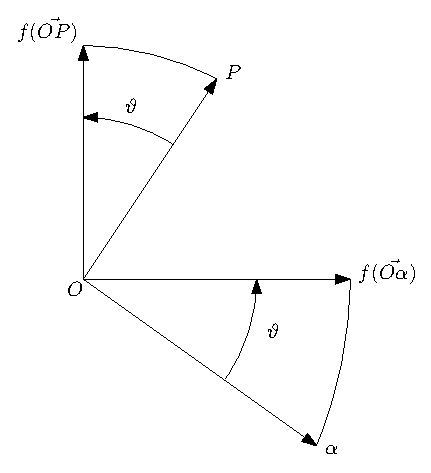
\includegraphics[width=5cm]{img/finiti/imgex4-2-1.eps}
      \caption{$f:V_O^2\to V_O^2$}
    \end{figure}
    Ora, come si vede nel disegno sequente, dati due vettori $\vec{OP}$ e $\vec{OP}^\prime$, sommarli e poi
    ruotare il vettore risultante oppure prima ruotarli e poi sommare i vettori ruotati è equivalente, ovvero
    \clearpage
    \begin{figure}[th]
      \centering
        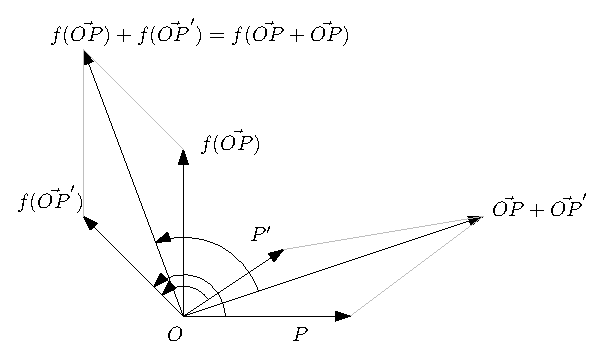
\includegraphics[width=6cm]{img/finiti/imgex4-2-2.eps}
      \caption{$f(\vec{OP})+f(\vec{OP}^\prime)=f(\vec{OP}+\vec{OP})$}
    \end{figure}
    Quindi vale la
    \begin{equation}
      f(\vec{OP})+f(\vec{OP}^\prime)=f(\vec{OP}+\vec{OP})
    \end{equation}
    che ci dice che questa funzione soddisfala proprietà (\ref{applin}) della Definizione \ref{4.1-4.2}\\
    Analogamente, dato un vettore $\vec{OP}$ e un numero reale $c$, moltiplicare il vettore per $c$ e poi
    ruotarlo e poi moltiplicarlo per $c$ è equivalente:
    \begin{figure}[th]
      \centering
        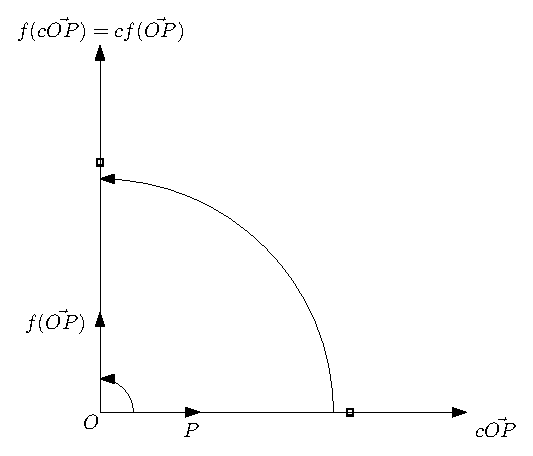
\includegraphics[width=6cm]{img/finiti/imgex4-2-3.eps}
      \caption{$f(c\vec{OP})=cf(\vec{OP})$}
    \end{figure}
    Quindi si ha
    \begin{equation}
      f(c\vec{OP})=cf(\vec{OP})
    \end{equation}
    che ci dice che questa funzione soddisfa anche la proprietà (\ref{matasapplin}), della definizione
    \ref{4.1-4.2} -- Concludiamo quindi che le rotazioni attorno a $O$ sono applicazioni lineari dallo
    spazio vettoriale $V_O^2$ in se stessso.\\
    Possiamo arrivare alla stessa conclusione anche per altre importanti trasformazioni geometriche: ad
    esempio, si consideri la riflessione rispetto a una retta $r$ passante per $O$, che manda ogni vettore
    $\vec{OP}\in V_O^2$ nel vettore simmetrico rispetto alla retta, come nel seguente disegno
    \begin{figure}[th]
      \centering
        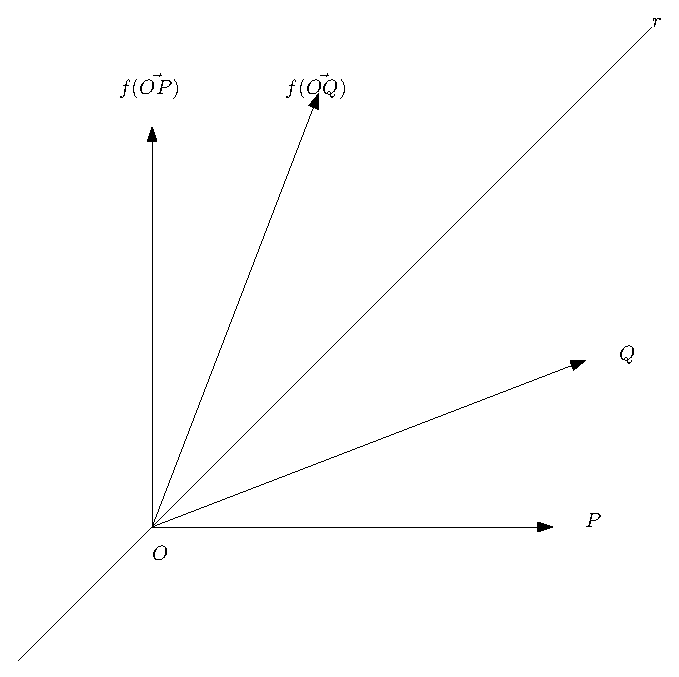
\includegraphics[width=6cm]{img/finiti/imgex4-2-4.eps}
    \end{figure}   
    Allora, come già fatto per le rotazioni, notiamo che, dati due vettori $\vec{OP}$ e $\vec{OP}^\prime$,
    sommarli e poi riflettere il vettore risultante oppure prima rifletterli e poi sommare i vettori riflessi
    è equivalente
    \clearpage
    \begin{figure}[th]
      \centering
        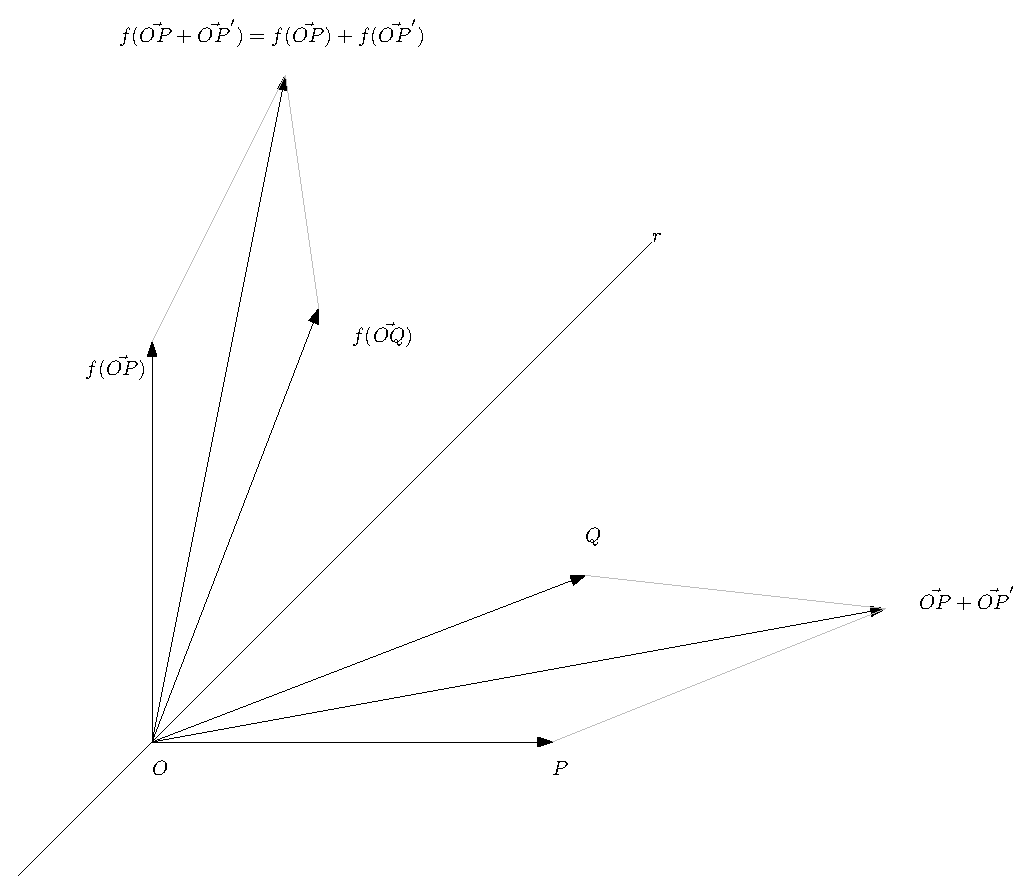
\includegraphics[width=6cm]{img/finiti/imgex4-2-5.eps}
    \end{figure}
    $f\left(\vec{OP}+\vec{OP}^\prime\right)=f\left(\vec{OP}\right)+f\left(\vec{OP}^\prime\right)$ e
    dato uin vettore $\vec{OP}$ e un numero
    reale $c$, moltiplicatore il vettore per $c$ e poi rifletterlo oppure prima rifletterlo e poi moltiplicarlo
    per $c$ è equivalente
    \begin{figure}[th]
      \centering
        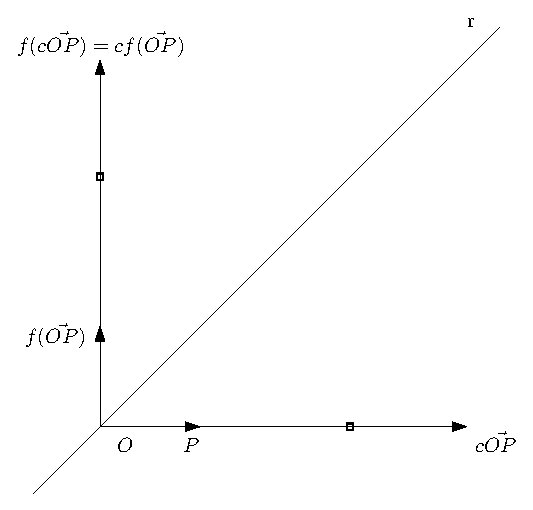
\includegraphics[width=6cm]{img/finiti/imgex4-2-6.eps}
    \end{figure}
      
    $f(c\vec{OP})=cf(\vec{OP})$: quindi concludiamo che anche la riflessione rispetto a una retta ce passa per
    $O$, avendo le proprietà entrambe le proprietà (\ref{4.1-4.2}) richieste nella Definizione (\ref{applin}),
    è un'applicazione lineare $f:V_O^2\to        V_O^2$.\\
    Come terzo esempio esempio di applicazione lineare $V_O^2\to V_O^2$ citiamo la propiezione ortogonale,
    che proieta ortogonalmente i vettori su una retta fissata passante per $O$.
    \begin{figure}[th]
      \centering
        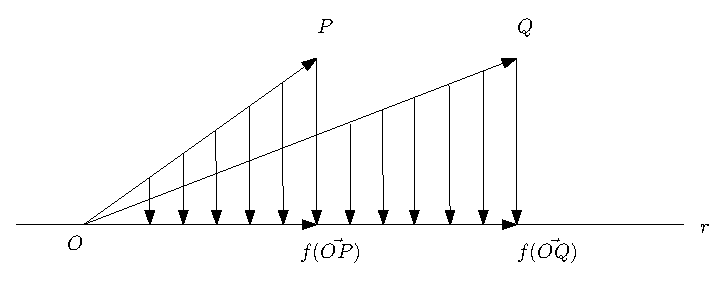
\includegraphics[width=8cm]{img/finiti/imgex4-2-7.eps}
    \end{figure}
      
    per la quale è difficile vedere che valgono ancora le proprieta citate in (\ref{4.1-4.2}).\\
    Analogamente a quanto visto per rotazioni, riflessioni e proiezioni nel piano, anche le corrispondenti
    trasformazioni $V_O^3\to V_O^3$ dello spazio tridimensionale come da proprietà (\ref{4.1-4.2}) della
    Definizione \ref{applin} la rotazione di un angolo fissato $\Theta$ attorno a una retta data passante per $O$
    (detta ase della rotazione)
    \clearpage
    \begin{figure}[th]
      \centering
        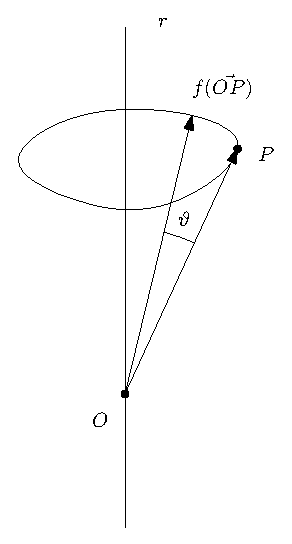
\includegraphics[width=3cm]{img/finiti/imgex4-2-8.eps}
    \end{figure}
    la riflessione rispetto a un piano passante per $O$
    \begin{figure}[th]
      \centering
        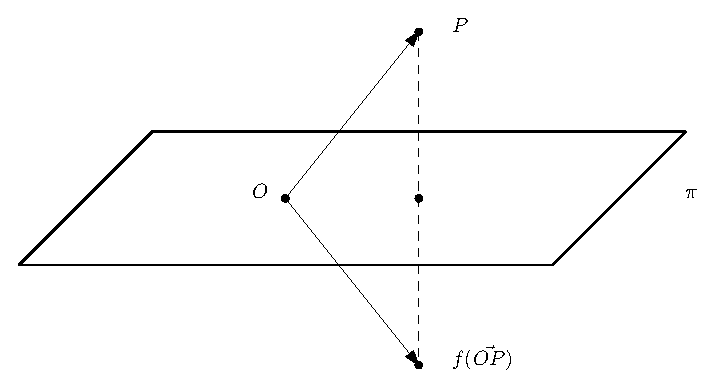
\includegraphics[width=6cm]{img/finiti/imgex4-2-9.eps}
    \end{figure}
      
    e la proiezione ortogonale su un piano passante per l'origine $O$:
    \begin{figure}[th]
      \centering
        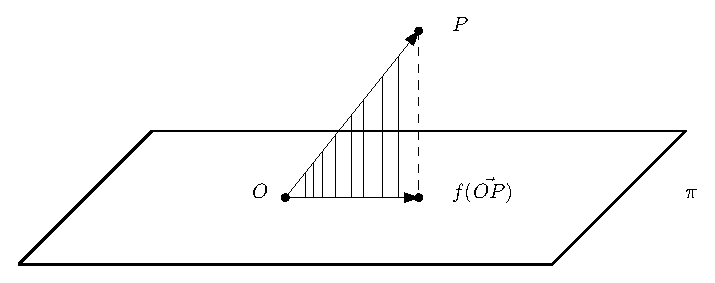
\includegraphics[width=6cm]{img/finiti/imgex4-2-10.eps}
    \end{figure}
    (Quest'ultima può anche essere vista come applicazione $f:V_O^3\to V_O^2$ se vediamo il piano su cui
    proiettiamo come spazio vettoriale a se stante).
  \end{esempio}
\end{definizione}

\section{Matrice associata a un'applicazione lineare}
Una delle caratteristiche fondamentali di un'applicazione lineare $f:V\to W$ è che, se gli spazi $V$ e $W$ hanno
dimensione finita, allora $f$ può essere rappresentata da una matrice.\\ Vediamo i dettagli: sia $f:V\to W$
un'applicazione lineare, e siamo $B_V=\left\{v_1,v_2,\dots,v_n\right\}$ e $B_W=\left\{w_1,w_2,\dots,w_n\right\}$
basi di $V$ e $W$ rispettivamente. Allora, come sappiamo ogni vettore $v\in V$ può essere identificato con una
$n-$upla $\left(x_1,x_2,\dots,x_n\right)$, quella delle sua coordinate rispetto alla base $B_V$ (ovvero
$v=x_1v_1+x_2v_2+\dots+x_nv_n$), e analogamente ogni vettore $w\in W$ può rispetto alla base $B_W$ (ovvero
$w=y_1w_1+y_2w_2+\dots+y_mw_m$). Con questo identificazioni, la $f$ può essere pensata come una funzione
$\mathds{K}^n\to\mathds{K}^m$ che associa a ogni $n$-upla. Ci proponiamo di trovare l'espressione esplicita di
tale funzione. A questo scopo, sia $(x_1,\dots,x_n)$ la $n$-upla delle coordinate di un vettore $v\in V$, ovvero
come abbiamo ricevuto sopra $v=x_1v_1+\dots+x_nv_n$. Allora la sua immagine $f(v)$ sarà
\begin{equation*}
  f(v)=f(x_1v_1+\dots+x_nv_n) =
\end{equation*}
(usando le proprietà un'applicazione lineare)
\begin{equation}
  =f(x_1v_1)+\dots+f(x_nv_n)=x_1f(v_1)+\dots+x_nf(v_n).
\end{equation}
Ora, ciascuno dei vettori $f(v_1),f(v_2),\dots,f(v_n)$ che compare nella ({\bf 4.5}) appartiene al codominio $W$
della funzione, e quindi potrà essere espresso come combinazione lineare dei vettori $w_1,w_2,\dots,w_m$ della
base $B_W$ fissata per $W$:
\clearpage
\begin{equation}
  f(v_1)=a_{11} w_1+a_{21}w_2+\dots+a_{m1}w_m
\end{equation}
\begin{equation*}
  \vdots
\end{equation*}
\begin{equation}
  f(v_1)=a_{1n} w_1+a_{2n}w_2+\dots+a_{mn}w_m
\end{equation}
Ora, sostituendo queste espressioni nella ({\bf 4.5}) si ottiene
\begin{equation*}
  f(v)=x_1(a_{11} w_1+a_{21}w_2+\dots+a_{m1}w_m) +\dots+ x_n(a_{1n} w_1+a_{2n}w_2+\dots+a_{mn}w_m)=
\end{equation*}
(svolgendo i conti e mettendo in evidenza i vettori)
\begin{equation}
  =(a_{11}x_1+\dots+a_{1n}x_n)w_1+\dots+(a_{m1}x_1+\dots+a_{mn}x_n)w_m
\end{equation}
Questa uguaglianza ci sta dicendo che le coordinate del vettore $f(v)$ rispetto alla base $B_W=\left\{w_1,w_2,
  \dots,w_m\right\}$ sono date da $a_{11}x_1+\dots+a_{1n}x_n,\dots,a_{m1}x_1+\dots+a_{mn} x_n$ e quindi che,
tradotta in coordinate, la nostra applicazione lineare può essere identificata con la funzione $\mathds{K}^n\to
\mathds{K}^m$ che associa a ogni $n$-upla $(x_1,\dots,x_n)$ la $m$-upla formata dai coefficienti che appiono nella
({\bf 4.8}), ovvero
\begin{equation}
  \begin{pmatrix}
    x_1\\
    x_2\\
    \vdots\\
    x_n
  \end{pmatrix} \to
  \begin{pmatrix}
    a_{11}x_1+a_{12}x_2+\dots+a_{1n}x_n\\
    a_{21}x_1+a_{22}x_2+\dots+a_{2n}x_n\\
    \vdots\\
    a_{m1}x_1+a_{m2}x_2+\dots+a_{mn}x_n
  \end{pmatrix}
\end{equation}
I coefficienti che compaiono nella ({\bf 4.9}) formano una matrice con $m$ righe e $n$ colonne
\begin{equation*}
  A=
  \begin{pmatrix}
    a_{11} &a_{12}&\dots&a_{1n}\\
    a_{21} & a_{22}&\dots& a_{2n}\\
    \dots\\
    a_{m1} & a_{m2} &\dots&a_{mn}
  \end{pmatrix}
\end{equation*}
che chiamaremo la \textit{matrice associata all'applicazione lineare rispetto alle basi $B_V$ e $B_W$}. In base
alle (\textbf{4.6}), \dots{}, (\textbf{4.7}) tale matrice può essere definita come \textit{la matrice che ha sulle
  colonne le coordinate dei vettori $f(v_1),\dots,f(v_n)$ (ovvero le immagini dei vettori della base $B_V$
  fissata nel dominio) rispetto alla base $B_W$ fissata nel codominio}.\\
Denoteremo $M_{B_wB_V}(f)$ la matrice associata a un'applicazione lineare $f:V\to W$ rispetto alle basi $B_V$ e
$B_W$.\\
Se dominio e codomio dell'applicazione coincidono, ovvero si ha una funzione linerare $f:V\to V$ (tale
applicazione si dicono \textit{endomorfismi}), allora è possibile fissare la stessa base $B_V$ sia nel dominio
che nel codominio, e calcolare la matrice associata $M_{B_wB_V}(f)$. Come vedremo, la matrice associata a
un'applicazione lineare ci dà tutte le informazioni di cui abbiamo bisogno sull'applicazione, e usando gli
strumenti imparati nei capitoli precedenti (\textit{rango, determinante}) saremo in grado di capire molte
proprietà della funzione data. Prima di fare ciò, vediamo subito alcuni esempi di calcolo della matrice
associata.
\begin{esempio}
  \begin{enumerate}
  \item Sia $f:V_O^2\to V_O^2$ la rotazione attorno a $O$ di un angolo fissato $\Theta$\footnote{abbiamo visto nel
      nel paragrafo precedente si tratta di un'applicazione lineare}. Per calcolare la matrice associata, fissiamo
    una base $B$ formata da due vettori $=v_1=\vec{OP}_1$ e $v_2=\vec{OP}_2$ dlla stessa lunghezza e
    perpendicolari tra loro, come nel disegno
    \begin{figure}[th]
      \centering
        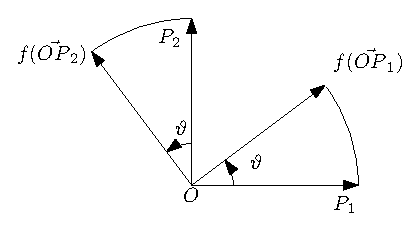
\includegraphics[width=6cm]{img/finiti/imgex4-3-1.eps}
    \end{figure}

    e determiniamo la matrice $M_B(f)$.\\
    A questo scopo, come afferma la difinizione di matrice associata dobbiamo trovare le coordinate di $f(v_1)$ e
    $f(v_2)$ rispetto a $B$, ovvero esprimere $f(\vec{OP}_1)$ e $f(\vec{OP}_2)$ come combinazione lineare
    $x_1\vec{OP}_1+x_2\vec{OP}_2$ dei vetori della base $B$. Iniziamo con $f(\vec{OP}_1)$: come si vede nel
    disegno seguente
    \clearpage
    \begin{figure}[th]
      \centering
        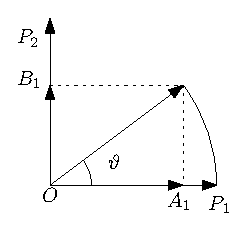
\includegraphics[width=6cm]{img/finiti/imgex4-3-2.eps}
    \end{figure}

    (nel quale stiamo denotando $R_1$ il punto finale del vettore ruotato $f(\vec{OP}_1)$) si ottine
    $f(\vec{OP}_1)=\vec{OP}_1=\vec{OA}_1+\vec{OB}_1$, essendo $A_1$ e $B_1$ le proiezioni ortogonali di $R_1$
    sui vettori di base. Ora, chiaramente $\vec{OA}_1=x_1\vec{OP}_1$ e $\vec{OB}_1=x_2\vec{OP}_2$, dove $x_1$ è
    dato dal rapporto $\frac{\abs{\vec{OA}_1}}{\vec{OP}_1}$ tra la lunghezza di $\vec{OA}_1$ e quella di
    $\vec{OP}_1$, mentre $x_2$ è dato dal rapporto $\frac{\abs{\vec{OB}_1}}{\vec{OP}_2}$ tra la lunghezza di
    $\vec{OB}_1$ e quella di $\vec{OP}_2$. Ma essendo la lunghezza di $\vec{OP}_1$ uguale alla lunghezza di
    $\vec{OR}_1=f(\vec{OP}_1)$\footnote{La rotazione non modifca la lunghezza dei vettore, essi restano
      inveriati anche se cambiano la loro angolazione.} possimo dire che $x_1$ è uguale al rapporto tra la
    lunghezza del cateto $\vec{OA}_1$ e quella dell'ipotenusa $\vec{OP}_1$ del triangolo rettangolo $OR_1A_1$,
    ovvero (esendo il cateto in questione adiacente all'angolo), $x_1=\cos\Theta$. \\
    Analogamente, poiché $\vec{OP}_1$ ha la stessa lunghezza di $\vec{OP}_1$ e quindi di $\vec{OR}_1$, mentre
    $\vec{OB}_1$ ha la stessa lunghezza del segmento $A_1R_1$, si ha 
    \begin{equation*}
      x_2=\frac{\abs{\vec{OB}_1}}{\abs{\vec{OP}_2}}=\frac{\abs{A_1R_1}}{OR_1}
    \end{equation*}
    ovvere\footnote{Essendo il rapporto tra il cateto $A_1R_1$, opposto all'angolo $\Theta$, e l'ipotenusa
      $OR_1$ del triangolo rettangolo $OR_1A_1$}, $x_2=\sin \Theta$. Riassumendo,
    \begin{equation}
      f(\vec{OP}_1)=\vec{OR}_1=\vec{OA}_1+\vec{OB}_1=\cos\Theta \vec{OP}_1+\sin \Theta \vec{OP}_2
    \end{equation}
    Ora, facciamo un ragionamento analogo per determinare $f(\vec{OP}_2)$: come si vede nel disegno seguente
    \begin{figure}[th]
      \centering
        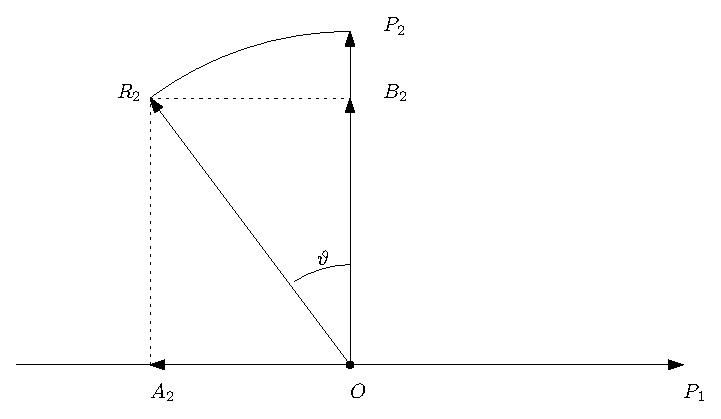
\includegraphics[width=6cm]{img/finiti/imgex4-3-3.eps}
    \end{figure}
      
    (nel quale stiamo denotando $R_2$ il punto finale del vettore ruotato $f(\vec{OPT})$) si ha
    $f(\vec{OP}_2)=\vec{OR}_2=\vec{OA_2}+\vec{OB_2}$. Ora, chiaramente $\vec{OA}_2=-x_1\vec{OP}_1$, dove $x_1$ è
    dato dal rapporto $\frac{\abs{\vec{OA}_2}}{\abs{\vec{OP}_1}}$ tra la lunghezza di $\vec{OA}_2$ e quella di
    $\vec{OP_1}$ (il segno meno è dovuto dal fatto che $\vec{OA}_2$ ha verso opposto rispetto a $\vec{OP}_1$) e
    $\vec{OB}_2=x_2\vec{OP}_2$, dove $x_2$ è dato dal rapporto $\frac{\abs{\vec{OB}_2}}{\abs{\vec{OP}_2}}$ tra la
    lunghezza di $\vec{OB}_2$ e quella di $\vec{OR}_2$. Ma essendo la lunghezza di $\vec{OP}_1$ uguale alla
    lunghezza di $\vec{OP}_1$ uguale alla lunghezza di $\vec{OP}_2$ e quindi di $\vec{OR}_2=f(\vec{OP}_2)$
    (sempre perché la rotazione non modifica la lunghezza dei vettori), mentre, la lunghezza di $\vec{OA}_2$ è
    uguale alla lunghezza del segmento $R_2B_2$, possiamo dire che $x_1$ è uguale al rapporto tra la lunghezza
    del cateto $R_2B_2$ e quella dell'ipotenusa $OR_2$ del triangolo rettangolo $OR_2B_2$, ovvero (essendo il
    cateto in questione opposto all'angolo), $x_2=\cos\Theta$.\\
    Riassumendo,
    \begin{equation}
      f(\vec{OP}_2)=\vec{OR}_2=\vec{OA}_2+\vec{OB_2}=-\sin\Theta\vec{OP}_1+\cos \Theta\vec{OP}_2
    \end{equation}
    \clearpage
    Quindi, (\textbf{4.10}) e (\textbf{4.11}) ci dicono che la matrice associata a $f$ rispetto a $B$ avrà sulla
    prima colonna $(\cos\Theta,\sin\Theta)$\footnote{le coordinate di $f(\vec{OP}_1)$ rispetto a $B$} e sulla
    seconda colonna $(-\sin\Theta,\cos\Theta)$ (le coordinate di $f(\vec{OP})$ rispetto a $B$), ovvero
    \begin{equation}
      M_B(f)=
      \begin{pmatrix}
        \cos\Theta & -\sin \Theta\\
        \sin\Theta & \cos \Theta
      \end{pmatrix}
    \end{equation}
    Come visto nel (\textbf{4.9}), abbiamo allora che la rotazione, in coordinate, si traduce nella funzione
    $f:\mathds{R}^2\to\mathds{R}^2$ data da
    \begin{equation}
      (x_1,x_2)\mapsto (\cos\Theta x_1-\sin\Theta x_2,\sin\Theta x_1+\cos\Theta x_2)
    \end{equation}
    Ad esempio, scegliamo $\Theta=\frac{\pi}{4}$ e sostituiamo in $(4.12)$ e $(4.13)$, ottenendo rispettivamente
    (si ricordi che $\cos\frac{\pi}{4}=\sin\frac{\pi}{4}=\frac{\sqrt{2}}{2}$)
    \begin{equation*}
      M_B(f)=
      \begin{pmatrix}
        \frac{\sqrt{2}}{2} & -\frac{\sqrt{2}}{2} \\
        \frac{\sqrt{2}}{2} & \frac{\sqrt{2}}{2}
      \end{pmatrix}.
    \end{equation*}
    e anche
    \begin{equation}
      (x_1,x_2)\mapsto
      \begin{pmatrix}
        \frac{\sqrt{2}}{2}x_1+\frac{\sqrt{2}}{2}x_2,\frac{\sqrt{2}}{2}x_1+\frac{\sqrt{2}}{2}x_2
      \end{pmatrix}
    \end{equation}
    Per illustrare come questa semplice funzione $\mathds{R}^2\to\mathds{R}^2$ rappresenti effettivamente la
    rotazione di $\frac{\pi}{4}$, prendiamo ad esempio il vettore $v=v_1+v_2$, che come si vede nel disegno
    seguente coincide con la diagonale del quadrato che ha $v_1$ e $v_2$ come lati:
    \begin{figure}[th]
      \centering
        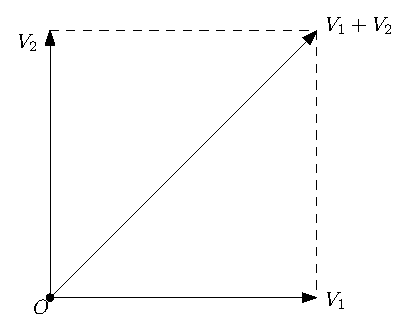
\includegraphics[width=4cm]{img/finiti/imgex4-3-4.eps}
    \end{figure}

    Tale vettore ha quindi come coordinate rispetto a $B$ la coppia $(x_1,x_2)=(1,1)$. In base alla
    \textbf{(4.14)}, le coordinate di $f(v)$ rispetto a $B$ sono date da
    \begin{equation*}
      \frac{\pi}{4}*1-\frac{\pi}{4}*1,\frac{\pi}{4}*1+\frac{\pi}{4}*1=(0,\sqrt{2})
    \end{equation*}
    ovvero deve essere $f(v)=0v_1+\sqrt{2}v_2=\sqrt{2}v_2$.\\
    In effetti, tale risultato ottenuto analicamente in coordinate è confermato dall'analisi grafica, che ci
    dice che il vettore $f(v)$ che si ottiene ruotando la diagonale $v$ del quadrato di $\frac{\pi}{4}$ è proprio
    proporzionale al vettore $v_2$ e la sua lunghezza è proprio $\sqrt{2}$ volte la lunghezza di $v_2$ (in
    quasto $v$ coincideva con la diagonale del quadrato di lati $v_1$ e $v_2$):
    \begin{figure}[th]
      \centering
        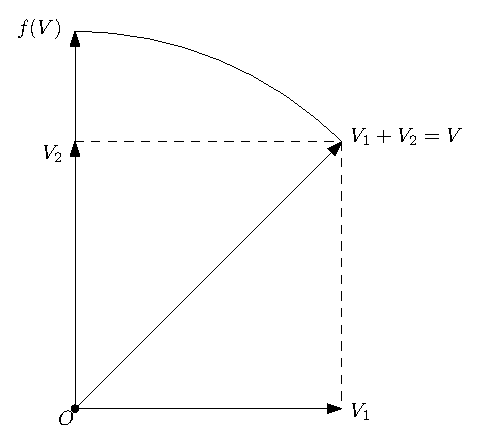
\includegraphics[width=4cm]{img/finiti/imgex4-3-5.eps}
    \end{figure}
  \item Sia $V=V_O^2$ lo spazio vettoriale dei vettori applicati in un punto $O$ nel piano e sia $f:V_o^2\to
    V_O^2$ la proiezione ortogonale su una retta fizzata $r$ passante per $O$\footnote{abbiamo visto nel
      paragrafo precedente che si tratta di un'applicazione lineare}.\\
    Ora, notiamo che quando proiettiamo $v_1$ ortogonalmente su $r$, otteniamo un vettore $v$ che sta sulla retta
    ed è lungo come metà della diagonale del quadrato i cui lati sono $v_1$ e $v_2$: essendo tale diagonale,
    per definizione di somma tra vettori, coincidente con $v_1+v_2$, abbiamo quindi che $f(v_1)=
    \frac{1}{2}(v_1+v_2)=\frac{1}{2}v_1+\frac{1}{2}v_2$; analogamente, come si vede dal disegno, anche
    proiettando $v_2$ sulla retta di ottiene lo stesso vettore $v$, quindi si ha anche $f(v_2)=
    \frac{1}{2}(v_1+v_2)=\frac{1}{2}v_1+\frac{1}{2}v_2$.
    \begin{figure}[th]
      \centering
        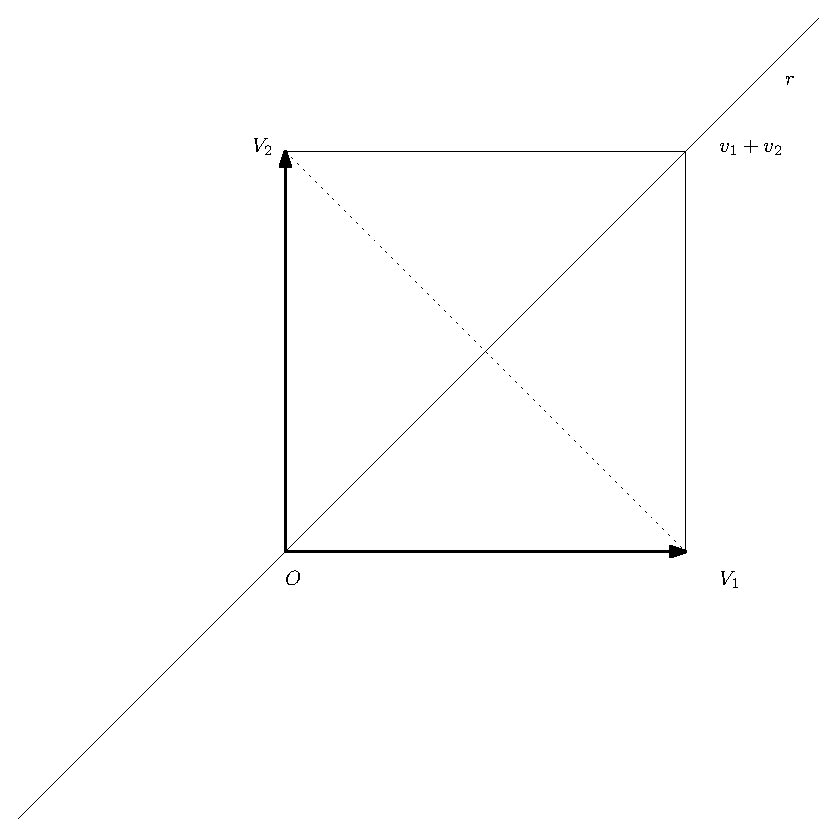
\includegraphics[width=4cm]{img/finiti/imgex4-3-6.eps}
    \end{figure}
    Si vede quindi che le coordinate di $f(v_1)$ rispetto a $B$ sono $\left(\frac{1}{2},\frac{1}{2}\right)$, e
    anche le coordnate di $f(v_2)$ rispetto a $B$ sono $\left(\frac{1}{2},\frac{1}{2}\right)$: disponendo tali
    coordinate rispettivamente sulla prima e sulla seconda colonna, come previsto dalla difinizione di matrice
    associata, si ottiene
    \begin{equation*}
      M_B(f)=
      \begin{pmatrix}
        \frac{1}{2}&\frac{1}{2}\\
        \frac{1}{2} & \frac{1}{2}
      \end{pmatrix}
    \end{equation*}
    e la funzione $\mathds{R^2}\to \mathds{R}^2$ corrispondente
    \begin{equation}
      (x_1,x_2)\mapsto
      \begin{pmatrix}
        \frac{1}{2}x_1+\frac{1}{2}x_2, \frac{1}{2}x_1+\frac{1}{2}x_2
      \end{pmatrix}
    \end{equation}
    ci dà una rappresentazione in coordinarte della proiezione.\\
    Ad esempio, il vettore $v=-v_1+v_2$, che ha coordinate $(-1,1)$ rispetto a $B$, viene mandata in base alla
    \textbf{(4.15)} nel vettore di coordinate
    \begin{equation*}
      \begin{bmatrix}
        \frac{1}{2}(-1)+\frac{1}{2}1, \frac{1}{2}(-1)+\frac{1}{2}1
      \end{bmatrix}=(0,0)
    \end{equation*}
    ovvero nel vettore nullo $\vec{OO}$. Infatti, come si vede dal seguente disegno, tale vettore appartiene
    alla retta passante per $O$ e ortogonale a $r$, e i vettori che giacciono su questa retta vengono chiaramnte
    proiettati sul vettore nullo $\vec{OO}$.
    \begin{figure}[th]
      \centering
        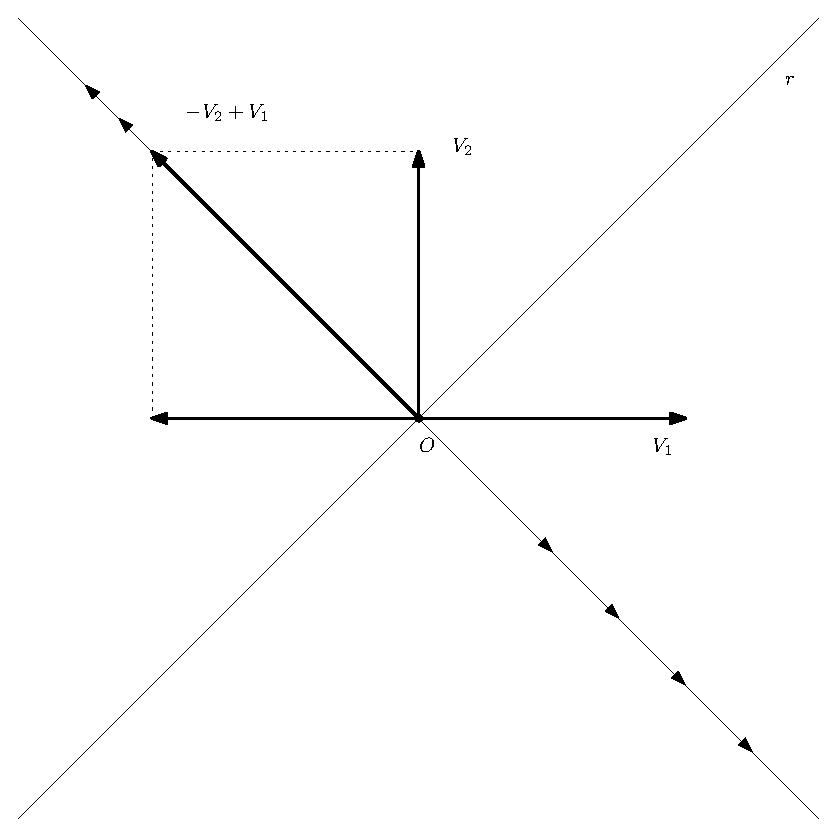
\includegraphics[width=6cm]{img/finiti/imgex4-3-7.eps}
    \end{figure}   
  \item Come ultimo esempio, prendiamo come funzione $f:V_O^2\to V_O^2$ la riflessione rispetto a una retta
    fissata $r$ passante per $O$, ovvero l'endomorfismo che associa a ogni vettore $\vec{OP}$ il suo simmetrico
    rispetto a $r$\footnote{Sappiamo dal primo paragrafo che si tratta di un'applicazione lineare}. Per calcolane
    la matrice associata $M_B(f)$, consideriamo la stessa base $B=\left\{v_1,v_2\right\}$ usata nell'esempio
    precedente.
    \clearpage
    \begin{figure}[th]
      \centering
        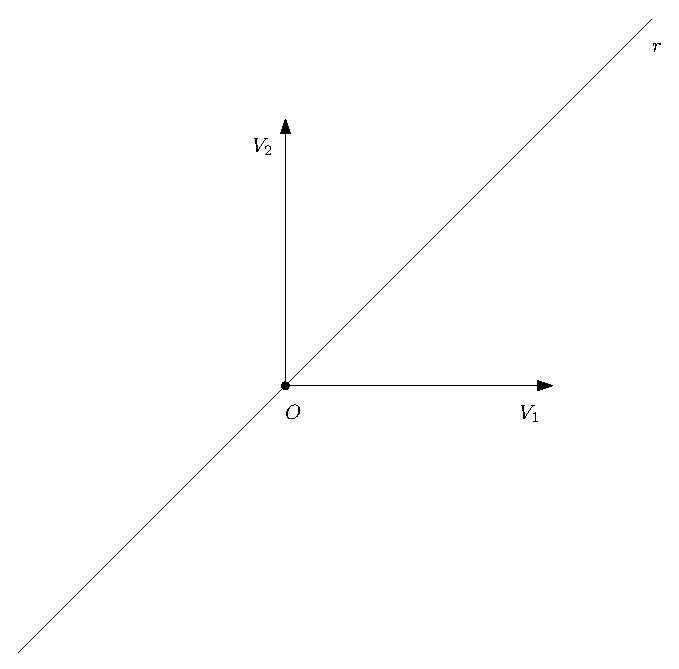
\includegraphics[width=4cm]{img/finiti/imgex4-3-8.eps}
    \end{figure}
    e notiamo che quando riflettiamo $v_1$ rispetto a $r$ otteniamo $v_2$, ovvero $f(v_1)=v_2$, analogamente
    quando riflettiamo $v_2$ rispetto a $r$, otteniamo $v_1$ ovvero $f(v_2)=v_1$.\\
    Quindi, riscrivendo $f(v_1)=v_2$ come $f(v_1)=0v_1+1v_2$ vediamo che le coordinate di $f(v_1)$ rispetto a $B$
    sono $(0,1)$, e analogamente riscrivendo $f(v_2)=v_1$ come $f(v_1)=1v_1+0v_2$ vediamo che le
    coordinate di $f(v_2)$ rispetto a $B$ sono $(1,0)$: disponendo tale coordinate in colonna,
    come previsto dalla definizione della matrice associata, si ottiene
    \begin{equation*}
      M_B(f)=
      \begin{pmatrix}
        0 & 1\\
        1 & 0
      \end{pmatrix}
    \end{equation*}
    Se dato sempre lo stesso endomorfismo, consideriamo invece la base $B^\prime= \{v_1^\prime,
    v^\prime_2$ come nel disegno seguente
    \begin{figure}[th]
      \centering
        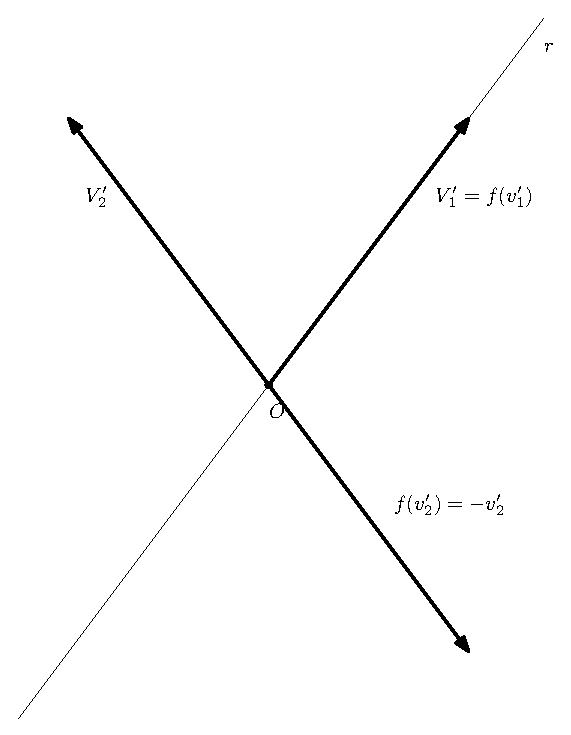
\includegraphics[width=4cm]{img/finiti/imgex4-3-9.eps}
    \end{figure}
    allora si ha che $f(v_1^\prime)=v_1^\prime$ (il vettore $v_1^\prime$ sta sulla retta e quindi
    la riflessione rispetto alla retta lo lascia invariato) e $f(v^\prime_2)=-v^\prime_2$ (il
    vettore $v_2^\prime$ è perpen dicolare alla fetta quindi riflettendolo esso cambia verso),
    cioè $f(v_1^\prime)=1v^\prime_1+0v^\prime_2$ e $f(v_2)=0v_1^\prime+(-1)v_2^\prime$ e quindi
     \begin{equation*}
      M_{B^\prime}(f)=
      \begin{pmatrix}
        1 & 0\\
        0 & -1
      \end{pmatrix}
    \end{equation*}
    Questo esempio illustra il fatto, ovvio che la matrice associata dipenda dalla scelta delle
    basi.
  \end{enumerate}
\end{esempio}

\section{Iniettività e suriettività delle applicazioni lineari}
\label{sec:inie_surie_app_lin}
Il primo problema che affronteremo sulla applicazioni lineari è determinare quando una tale
funzione è iniettiva, suriettiva o biiettiva.

\subsection{Richiami generali}
\label{sec:inie_surie_app_lin_ric_gen}
Ricordiamo che una funzione $f:A\to B$ tra due insiemi $A$ e $B$ si dice \textit{suriettiva} se
ogni elemento del codominio $B$ risulta essere immagine di qualche elemento di $A$ (ovvero, se
per ogni $b\in B$ esiste un $a\in A$ tale che $f(a)=b$).\\
Ad esempio, delle funzioni rappresentate nel seguente disegno, la prima non è
suriettiva\footnote{L'elemento $c\in B$ non è immagine di nessun elemento di $A$},
mentre, la seconda si.
\begin{figure}[th]
  \centering
  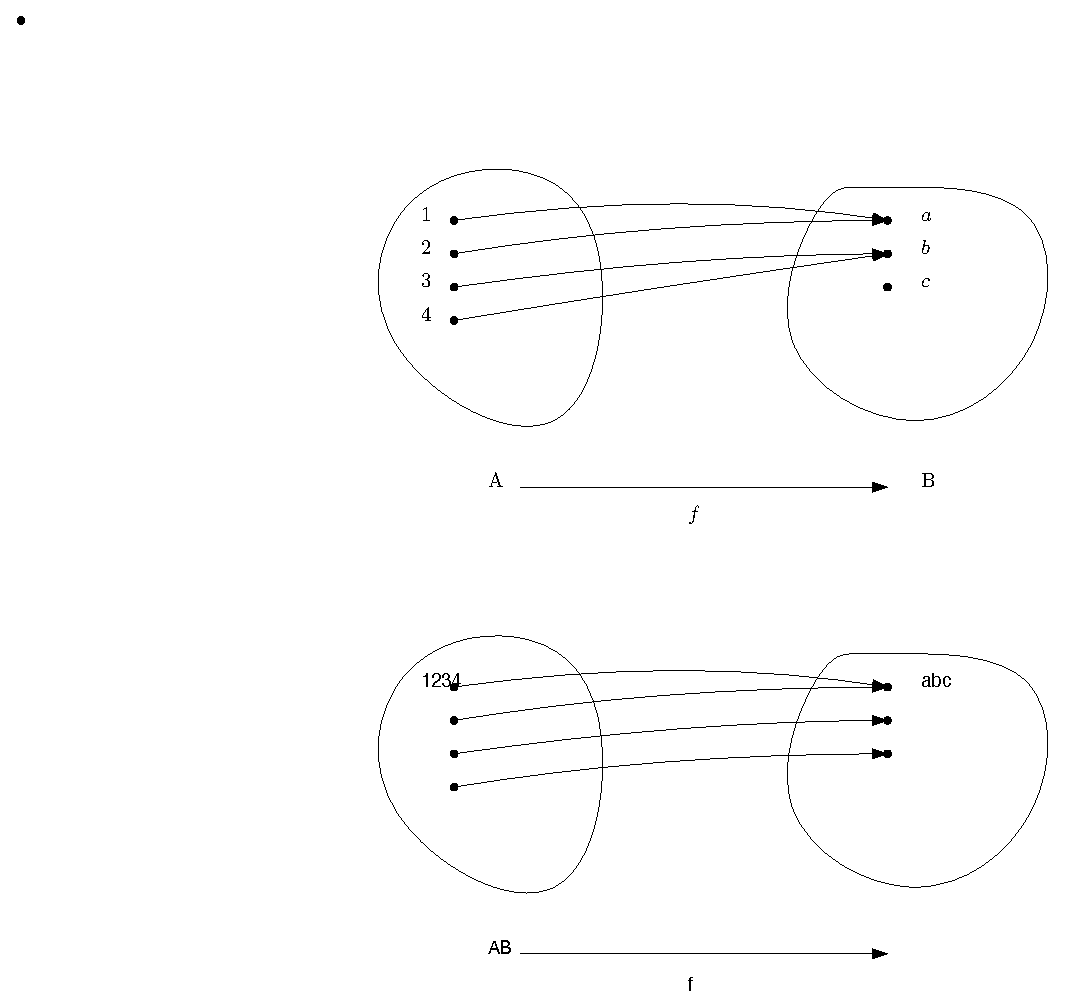
\includegraphics[width=8cm]{img/finiti/imgex4-4-1.eps}
  \caption{differenza tra iniettivo e suriettivo}
\end{figure}
Un modo alternativo di dire che una funzione èsuriettiva è fare riferimento alla cosidetta 
\textit{immagine} $I_m(f)$ di f: per definizione, l'immagine di una funzione $f:A\to B$ è il
sottoinsieme di $B$ costituito da futti gli elementi che sono immagine di qualche elemento di $A$
(in riferimento ai disegni, quegli elementi ``raggiunti da una freccia che provviene da A''),
ovvero
\begin{equation*}
  I_m(f)=\{b\in B | b=f(a) \text{ per qualche } a \in A\}
\end{equation*}
Ad esempio, la funzione sopra nel disegno precedente ha $I_m(f)=\{a,b\}$, mentre la funzione
sotto ha $I_m(f)=\{a,b,c\}$ç una funzione è suriettiva esattamente quando $I_m(f)=B$, ovvero
l'immagine coincide con tutto il codominio\footnote{Dire $I_m(f)=B$ significa in effetti dire
  che ogni elemento di $B$ è immagine di quelche elemento di $A$}.
\begin{figure}[th]
  \centering
  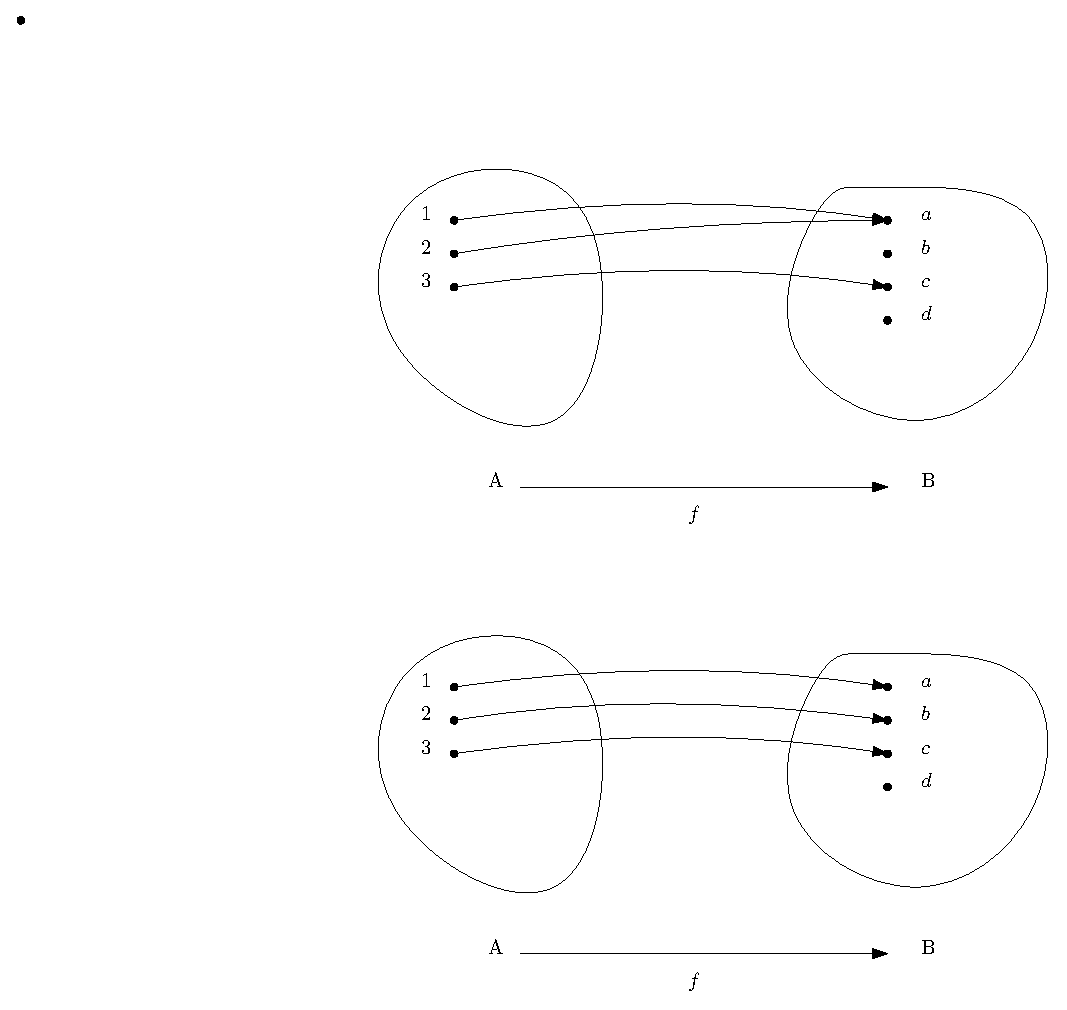
\includegraphics[width=8cm]{img/finiti/imgex4-4-2.eps}
\end{figure}

La nozione di iniettività può essere riformata tramite il concetto di \textit{controimmagine}:
dato un elemento $b$ del codomiono $B$, la sua controimmagine, denotata $f^{-1}(b)$, è l'insieme
di tutti gli elementi di $A$ che hanno $b$ come immagine, ovvero
\begin{equation*}
  f^{-1}(b)=\{a\in A|f(a)=b\}
\end{equation*}
Dal momento che una funzione è iniettiva quando non esistono dhe elementi diversi che hanno la
stessa immagine, dire che una funzione è iniettiva quivale a dire che tutte le controimmagini
che non siano vuote\footnote{se la funzione non è suriettiva, ci saranno elementi $b\in B$ tali
  che non esiste nessun $a\in A$ con $f(a)=b$ e quindi la cui controimmagine $f^{-1}(b)$ non ha
  elementi.} hanno un solo elemento.\\
Ad esempio, per la funzione sofra nel disegno precedente si ha $f^{-1}(a)=\{1,2\},f^{-1}(b)=
\not{0},f^{-1}(c)=\{3\}$: essa non è iniettiva in quanto la controimmagine di a ha due elementi.\\
Per la funzione sotto, invece, si ha $f^{-1}(a)=\{1\}, f^{-1}(b)=\{2\},f^{-1}(c)=\{3\},
f^{-1}(d)=\not{0}$: essa è iniettiva in quanto le controimmagini non vuote hanno tutte un solo
elemento.\\
Infine, una funzione si dice \textit{biiettiva} se è sia inittiva che suriettiva. Ad esempio,
la funzione rappresentata nel sequente disegno è biiettiva.
\begin{figure}[th]
  \centering
  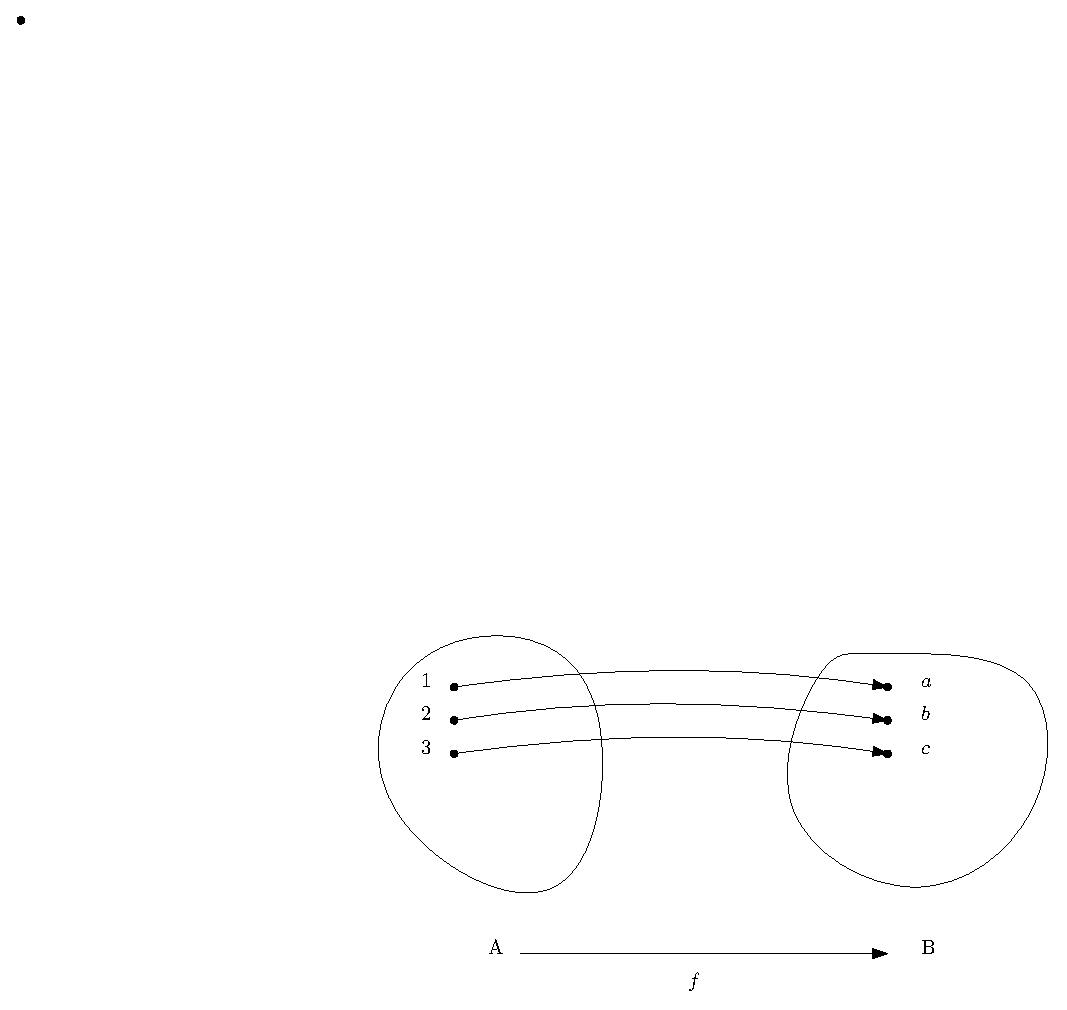
\includegraphics[width=8cm]{img/finiti/imgex4-4-3.eps}
\end{figure}

\subsection{Suriettività delle applicazione lineari}
Abbiamo detto che una funzione $f: A\to B$ è suriettiva se e solo se per ogni elemento di
$b\in B$ esiste un $a\in A$ tale che $f(a)=b$, ovvero equivalentemente se e solo se la sua
immagine $I_m(f)$ coincide con tutto il codominio.\\
Nel caso di un'applicazione lineare $f:V\to W$, vale la seguente importante
\begin{proposizione}
  Sia $f: V\to W$ un'applicazione lineare. Allora $I_m(f)$ è un sottospazio vettoriale di W.
\end{proposizione}
\begin{proof}
  Dobbiamo verificare che $I_m(f)$ è chiuso rispetto alla somma e al prodotto per scalari. Per la
  prima proprietà dobbiamo prendere $w,w^\prime\in I_m(f)$ e vedere se $w+w^\prime\in I_m(f)$. Ora,
  se $w,w^\prime\in I_m(f)$, per definizione di $I_m(f)$ significa che esistono un vettore
  $v\in V$ tale che $w=f(v)$ e un vettore $v^\prime\in V$ tale che $w^\prime=f(v^\prime)$ e un
  vettore $v^\prime\in V$ tale che $w=f(v)$ e un vettore $v^\prime \in V$ tale che
  $w^\prime\in f(v^\prime)$. Ma allora, sfruttando il fatto che $f$ è lineare, si ha
  \begin{equation*}
    w+w^\prime=f(v)+f(v^\prime)=f(v*v^\prime)
  \end{equation*}
  che ci dice che anche $w+w^\prime$ è immagine di un elemento del dominio (cioè $v+v^\prime$) e
  quindi $w+w^\prime\in m(f)$.\\
  Per la chiusura rispetto al prodotto per scalari, dobbiamo verificare che se $w\in I_m(f)$ e
  $c\in\mathds{K}$, allora $cw\in I_m(f)$. Ma, come prima, se $w\in I_m(f)$ allora per
  definizione di $I_m(f)$ esiste un vettore $v\in V$ tale che $w=f(v)$, e quindi, usando sempre
  il fatto che $f$ è linerare,
  \begin{equation*}
    cw=cf(v)=f(cv)
  \end{equation*}
  che ci dice che anche $cw$ è immagine di un elemento del dominio (cioè $cv$) e quindi $cw\in I_m(f)$.
\end{proof}
Il fatto che $I_m(f)$ sia un sottospazio vettoriale ci dice che per determinarla possiamo trovarne un sistema di
generatori o una base. Questo si fa facilmente grazie alla seguente
\begin{proposizione}
  Sia $f:V\to W$ un'applicazione lineare e siamo $v_1,\dots,v_n$ generatori $V$.
  Allora le immagini $f(v_1),\dots,f(v_n)$ generano $I_m(f)$ (in simboli, $I_m(f)=[f(v_1),\dots,f(v_n)]$)
\end{proposizione}
\begin{proof}
  Per definizione di generatori, dobbiamo verificare che ogni vettori $w\in I_m(f)$ si può scrivere come
  combinazione lineare dei vettori $f(v_1),\dots,f(v_n)$. Ora, sappiamo che un vettore $w\in I_m(f)$ è tale che
  $w\in f(v)$ per qualche $v\in V$. Ma essendo per ipotesi $v_1,\dots,v_n$ generatori di $V$, il vettore
  $v$ potrà essere scrittocome loro combinazione lineare $v=x_1v_1+\dots+x_nv_n$. Quindi, sfruttando la
  linearità di $f$ si ha
  \begin{equation*}
    w=f(v)=f(x_1v_1+\dots+x_nv_n)=x_1f(v_1)+\dots+x_nf(v_n)
  \end{equation*}
  che dimostra prprio che $w$ si scrive come combinazione lineare di $f(v_1),\dots,f(v_n)$, come volevamo.
\end{proof}
A questo punto, per determinare se un'applicazione lineare $f:V\to W$ è suriettiva, basta scegliere dei
generatori $v_1,\dots,v_n$ di $V$, prendere le loro immagini $f(v_1),\dots,f(v_n)$ che, come abbiamo appena
visto, formano un insieme di generatori di $I_m(f)$, e poi estrarre da quest'ultimo insieme una base eliminando
gli eventuali vettori che sono dipendenti dai rimanenti: contando i vettori della base ottenuta, sapremo la
dimensione di $I_m(f)$ e quindi $f$ sarà suriettiva se e solo se\footnote{Questa affermazione è giustificato
  dal fatto, che non abbiamo dimostrato, che se $S$ è un sottospazio vettoriale di una spazio vettoriale $V$,
  allora $dim (S)\leq dim (V)$ e le dimensioni coincidono se e solo se $S=V$.} $dim(I_m(f))=dim(W)$.\\
Vediamo come tale criterio di suriettività si rivela particolarmente utile e di semplice applicazione nel caso
dell'applicazioni lineare $L_A:\mathds{K}^n\to \mathds{K}^m$ determinata da una matrice $A$, ovvero della forma
data dalla (4.9)\footnote{Come sappiamo, ogni applicazione lineare puo`essere identificata con una tale
  funzione grazie alla matrice associata}.\\
Ora, se come generatori del dominio $V=\mathds{K}^n$ scegliamo i vettori della base canonica
$v_1=(1.0.\dots,0),v_2=(0,1,\dots,0),v_n=(0,0,\dots,1)$, dalla (4.9) si ha
\begin{equation*}
  f(v_1)=L_A
  \begin{pmatrix}
    1 \\
    0 \\
    \vdots\\
    0
  \end{pmatrix}=
  \begin{pmatrix}
    a_{11}\\
    a_{12}\\
    \vdots\\
    a_{m1}
  \end{pmatrix},
  f(v_2)= L_A
   \begin{pmatrix}
    0 \\
    1 \\
    \vdots\\
    0
   \end{pmatrix}=
   \begin{pmatrix}
    a_{12}\\
    a_{22}\\
    \vdots\\
    a_{m2}
   \end{pmatrix}, \dots, f(v_n)=
   L_A
   \begin{pmatrix}
    0\\
    0\\
    \vdots\\
    1
   \end{pmatrix}=
   \begin{pmatrix}
    a_{1n}\\
    a_{2n}\\
    \vdots\\
    a_{mn}    
   \end{pmatrix}
\end{equation*}
cioè $f(v_1),f(v_2),\dots,f(v_n)$ sono le colonne $C_1,C_2,\dots,C_n$ della matrice $A$ che determina
l'applicazione. Quindi, in base alla Proposizione \textbf{2}, si ha $I_m(f)=\{C_1,c_2,\dots,C_n\}$ e la funzione
è suriettiva se e solo se $dim\{C_1,C_2,\dots,C_n\}=dim(\mathds{K}^m)=m$. Ma poiché la dimensione del sottospazio
generato dalle colonne di una metrice è per definizione il suo rango, concludiamo che \textit{un'applicazione
  del tipo (4.9) è suriettiva se e solo se il rango di $A$ è uguale a $m$}.

\subsection{Iniettività di applicazioni lineari}
Mentre nel caso della suriettività abbiamo visto che per verificare se una funzione $f$ è suriettiva basta
controllare un solo sottoinsieme del codomonio (l'immagine $I_m(f)$), in generale per verificare se $f$ è
iniettiva dobbiamo a priori controllare tutte le controimmagini degli elementi del codominio e verificare che
queste, quando non sono vuote, hanno un solo elemento.\\
Ora, per una generica funzione $f:A\to B$ le controimmagini degli elementi di $B$ sono sottoinsiemi del tutto
indipendenti tra loro: come nel seguente disegno
\begin{figure}[th]
  \centering
  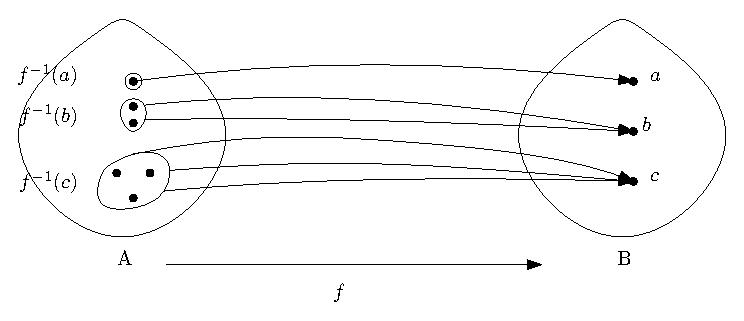
\includegraphics[width=8cm]{img/finiti/imgex4-4-4.eps}
\end{figure}

può accadere che un elemento abbia controimmagine costituine costituita da un solo elemento ma altri abbiamo
controimmagine costituita da più elementi. Vedremo ora invece che le applicazioni lineari hanno il particolare
comportamento per cui le controimmagini degli elementi di $B$, se non sono vuote, o sono \textit{tutte}
costituite da un solo elemento (nel quel caso la funzione non è iniettiva): quindi basta controllare una sola
controimmagine non vuota per capire come sono fatte tutte le altre. Più precisamente abbiamo la seguente
\begin{proposizione}
  Sia $f: V\to W$ un'applicazione lineare. Allora valgono i seguenti fatti:
  \begin{description}
  \item[(i)] la controimmagine $f^{-1}(\bar{0})=\{v\in V | f(v)=\bar{0}\}$ del vettore nullo di $W$ è un
    sottomatrice vettoriale di $V$ (detto \textit{nucleo di} $f$ denotato $N(f)$)
  \item[(ii)] per ogni $w_0\in W$, la controimmagine $f^{-1}(w_0)$ di $w_0$,  non è vuota, è un sottospazio
    affine di $V$, e più precisamente
    \begin{equation*}
      f^{-1}(w_0)=v_0+N(f)=\{v_0+n|n\in N(f)\}
    \end{equation*}
    dove $v_0$ è un qualunque elemento fissato d $f^{-1}(w_0)$.
  \end{description}
\end{proposizione}
\begin{proof}
  Per dimostrare $(i)$, iniziamo con l'osservare che il nucleo di $f$ non è mai vuoto, in quanto il vettore
  nullo di $V$ (che, con un abuso di notazione, denotiamo ancora $\bar{0}$) è sicuramente tale che
  $f(\bar{0})=\bar{0}$: infatti, possiamo il vettore nullo $\bar{0}$ di $V$ come $0v$ (dove $v$ è un qualunque
  vettore di $V$) e quindi, sfruttando la linearità di $f$, si ha $f(\bar{0})=f(0v)=0f(v)=\bar{0}$.\\
  Siano $v,v^\prime$ due vettori di $N(f)$, cioè $f(v)=\bar{0}$. Allora, essendo $f$ lineare,
  \begin{eqnarray*}
    f(v+v^\prime)=f(v)+f(v^\prime)=\bar{0}+\bar{0}=\bar{0}
  \end{eqnarray*}
  e quindi anche $v+v^\prime\in N(f)$: questo ci dice che $N(f)$ è chiuso rispetto alla somma.
  Dati invece un vettore $v$ del nucleo\footnote{quindi $f(v)=\bar{0}$} e uno scalare $c\in
  \mathds{K}$, allora, sempre per la linearità di $f$,
  \begin{eqnarray*}
    f(cv)=cf(v)=c\bar{0}=\bar{0}
  \end{eqnarray*}
  ovvero $cv\in N(f)$: questo ci dice che $N(f)$ chiuso rispetto al prodotto per scalari -- La
  \textit{(i)} è dimostrata.\\
  Per dimostrare la \textit{(ii)}, ovvero l'ugualianza $v=N(f)=f^{-1}(w_0)$, dobbiamo dimostrare
  che ogni elemento di $v_0+N(f)$ sta nella controimmagine $f^{-1}(w_0)$ appartiene a $v_0+N(f)$
  (ovvero l'inclusione opposta $f^{-1}(w_0)$). Per dimostrare la prima inclusione, consideriamo il
  generico elemento di $v_0=N(f)$, cioè, per definizione di sottospazio affine, un vettore $v$ del
  tipo $v=v_0+n$, con $n\in N(f)$. Allora
  \begin{equation*}
    f(v)=f(v_0+n)=f(v_0)+f(n)=f(v_0)=\bar{0}=f(v_0)=w_0
  \end{equation*}
  (nella seconda uguaglianza abbiamo usato il fatto che $f$ è lineare, nella terza il fatto che $n$ appartiene
  al nucleo di $f$ e quindi $f(n)=\bar{0}$). Abbiamo dimostrato che $f(v)=w_0$, cioè $v$ appartiene alla
  controimmagine $f^{-1}(w_0)$ di $w_0$, come volevamo.\\
  Per dimostrare la seconda inclusione, consideriamo un qualunque elemento $v$ della controimmagine di $w_0$,
  cioè $f(v)=w_0$. Essendo $w_0=f(v_0)$, si ha quindi $f(v)=f(v_0)$, da cui, portando a primo membro,
  $f(v)-f(v_0)=\bar{0}$. Essendo $f$ lineare, quest'ultima uguaglianza può essere riscritta $f(v-v_0)=\bar{0}$,
  il che ci dice che il vettore $v-v_0$ appartiene al nucleo $N(f)$ di $f$. Ma allora, osservando che chiaramente
  $v=v_0+(v-v_0)$, vediamo che $v$ si decompone proprio come somma di $v_0$ e di un elemento del nucleo $N(f)$,
  $v\in v_0+N(f)$, come volevamo.
\end{proof}

\end{document}

